\documentclass[15pt,letterpaper]{article}

\PassOptionsToPackage{hyphens}{url}

\usepackage{booktabs}
\usepackage{caption}

\usepackage{setspace}
\doublespacing
\usepackage[]{natbib}
\bibliographystyle{apalike}
% \bibliographystyle{plainnat}

% === MARGINS ===
\addtolength{\hoffset}{-0.75in} 
\addtolength{\voffset}{-1.25in}
\addtolength{\textwidth}{1.5in} 
\addtolength{\textheight}{2.25in}

% == ENVS ==
\newenvironment{tightcenter}{%
  \setlength\topsep{0pt}
  \setlength\parskip{0pt}
  \begin{center}
}{
  \end{center}
}

% == PACKS ==
\usepackage{color,soul}
\usepackage{graphicx} % to use pngs in tex (include graphix)
\usepackage{calc} % To scale \pagewidth with \real{float}
\usepackage{pgfplots} % To draw histogram

\pgfplotsset{
  compat=1.17, 
colormap/viridis
} % request specific version of pgfplots

\usepackage{calc} % to use \real for text -> numeric
\usepackage{pgf} % to store numeric variables
\usepackage{subcaption} % to place two figures horizontally
\usepackage{caption} % to refer subfigure
\renewcommand{\thesubfigure}{(\alph{subfigure})}
\captionsetup[sub]{labelformat=simple}
\captionsetup[table]{font={stretch=1.2}}  % adjust line space in captions of TABLE and FIGURES
\captionsetup[figure]{font={stretch=1.2}}  


\usepackage{tikz}
\usetikzlibrary{automata,positioning}
\usetikzlibrary{arrows.meta, positioning, automata}
\usetikzlibrary{spy}
\usetikzlibrary{shadows}
\usetikzlibrary{arrows,positioning,shapes.geometric} % for dnn flowchart


\tikzset{
  font={\fontsize{10pt}{0}\selectfont}}
\usepackage{forest}
\tikzset{
  Decision/.style = {%
    draw,
    line width=1.4pt
  },
  Lottery/.style = {%
    draw,
    line width=1.4pt
  },
  Outcome/.style = {%
    circle,
    minimum width=3pt,
    fill,
    inner sep=0pt
  }
}
\usepackage{csquotes}
\usepackage{lipsum}
\usetikzlibrary{arrows.meta,automata,positioning} % to draw directed-weighted-graph


\usepackage{amsmath, amssymb, latexsym} % NN
\usepackage{tikz}% NN
\usetikzlibrary{decorations.pathreplacing}% NN
\usetikzlibrary{fadings}% NN


\usepackage{xltabular}
\usepackage{booktabs}

\usepackage[breakable, skins]{tcolorbox} % to add factual asepct inside a frame

\usepackage[title]{appendix}

%to prevent page and footnotes swalloen by the table


% == Checkmarks == 
\usepackage{bbding}
\usepackage{pifont}
\usepackage{wasysym}
\usepackage{amssymb}
% ================

% == BIBS ==
% \usepackage{natbib}

\usepackage{diagbox}

\usepackage[bottom]{footmisc}

\usepackage[
  hidelinks,
  pdftex, 
  bookmarksopen=true, 
  bookmarksnumbered=true,
  pdfstartview=FitH, 
  breaklinks=true, 
  urlbordercolor={0 1 0}, 
  citebordercolor={0 0 1}]
  {hyperref}

\usepackage[ruled,vlined,linesnumbered]{algorithm2e}
\SetKwFor{For}{for (}{) $\lbrace$}{$\rbrace$}

%%% Coloring the comment as blue
\newcommand\mycommfont[1]{\footnotesize\ttfamily\textcolor{blue}{#1}}
\SetCommentSty{mycommfont}

\SetKwInput{KwInput}{Input}                % Set the Input
\SetKwInput{KwOutput}{Output}   
\usepackage{algpseudocode}% http://ctan.org/pkg/algorithmicx
\usepackage{varwidth}% http://ctan.org/pkg/varwidth


\usepackage{titlesec}

\setcounter{secnumdepth}{4}

\titleformat{\paragraph}
{\normalfont\normalsize\bfseries}{\theparagraph}{1em}{}
\titlespacing*{\paragraph}
{0pt}{3.25ex plus 1ex minus .2ex}{1.5ex plus .2ex}


% == SPACES == 

% == CMMDS ==
\newcommand{\tit}{
\Large \bf
Decoding the Congressional Portfolio: Unveiling Industry Specialization in Congresspersons' Stock Trading Through Graph Neural Networks
}
\newcommand\spacingset[1]{\renewcommand{\baselinestretch}
{#1}\small\normalsize}

% To draw embedding layer
\newcommand*{\xMin}{0}%
\newcommand*{\xMax}{6}%
\newcommand*{\yMin}{0}%
\newcommand*{\yMax}{9}%
% To draw conv output
\newcommand*{\xMinOut}{10}%
\newcommand*{\xMaxOut}{11}%
\newcommand*{\yMinOut}{1}%
\newcommand*{\yMaxOut}{8}%


% == VARS == 
\pgfmathsetmacro{\heatmap}{1}

\makeatletter
\setlength{\@fptop}{0pt}
\makeatother

% == START (PageCounter, Mode)
\begin{document}

\spacingset{1.25}

\setcounter{page}{0}
\vspace{-.1in}

% == TITLE (includes DraftDate)
{\title{
    \tit
  }
  \author{
    Suyeol Yun
  \thanks{PhD Student, Department of Political Science, MIT. Email: \href{mailto:syyun@mit.edu}{syyun@mit.edu}\\
  % **The reproducible code and data can be found at the following link: \href{https://github.com/syyunn/efd}{https://github.com/syyunn/efd}.
  }
  }
  \maketitle
}

\thispagestyle{empty}
\vspace{-.1in}

\begin{abstract}

  In this paper, I reassess a specific claim made in a previous study that a U.S. Congressperson’s stock trading behavior is not significantly associated with their committee assignments. Instead, I present evidence to support the notion that Congresspersons demonstrate an industry specialization in their stock trading, which tends to align with the industries relevant to their committee assignments. This alignment suggests that, whether intentional or unconscious, a Congressperson's legislative specialization can influence their personal financial decisions.
  My analysis, conducted using graph neural networks on a graph-structured dataset that captures a range of legislative activities, confirms that the excess return of Congresspersons is not widespread, but rather confined to a select few. This finding provides compelling evidence that Congresspersons' stock trading is primarily based on an industry-level understanding, rather than specific firm-level information.  
  To unravel this complex relationship, I apply the Graph Neural Network Explainer, an algorithm designed to demystify the inner workings of neural networks. By performing an ablation study on the predictions made by the Graph Neural Network, I identify which types of congressional activities are most influential in predicting stock trading behavior.  
  My findings challenge the assumptions of the specific prior study and present a more nuanced understanding of Congressional stock trading behavior. This study adds depth to our understanding of the intersection between financial interests and legislative roles, suggesting the need for more comprehensive research and policy considerations regarding financial ethics in public service.
  
\end{abstract}
\clearpage

% == INTRO ==
\section{Introduction}
\spacingset{2} % gives a slightly more margin between abstract and introduction
% [MOTIVATION]

In democratic societies, electoral accountability is a central mechanism through which politicians, vested with the power to make significant public decisions, remain answerable for their actions (Besley 2006, Fearon, 1999 Ferejohn, 1986). However, the intermingling of public service and personal financial interests can blur the lines of accountability. A key question arises: how closely intertwined are a politician's personal financial gains and their public service role? Are these two realms neatly partitioned, or do they bleed into each other?

The moral hazard theory raises concerns that when individuals are shielded from the repercussions of their actions, they might behave differently than if they bore the full consequences (Holmstrom, 1979). This theory is especially pertinent in the political sphere, where politicians could leverage their positions for personal financial gains, leading to potential conflicts of interest. The theory underscores the need for a deeper theoretical and empirical examination of politicians' behavior in this regard. 

Public choice theory, in addition, posits that it is unrealistic to presume a clear-cut divide between the public and private domains of a politician's life (Buchanan and Tollison, 1984). The theory suggests that individuals aim to maximize their personal utility in both their public and private roles. This notion aligns with Fenno's home style approach, which suggests that personal interests can often shape political actions aimed at re-election (Fenno, 1973).

Given these theoretical considerations, the financial behavior of politicians, particularly their stock trading activities, warrants closer examination. The trading activities of U.S. Congresspersons offer a unique opportunity to investigate the relationship between public service and personal financial interests. By analyzing the stock trading patterns of Congresspersons and their legislative activities, we can gain valuable insights into the potential conflicts of interest and the implications for electoral accountability.
The issue of financial behavior among politicians has been explored from various angles. Legal scholars have examined the use of political intelligence for profit and the potential for insider trading within the political sphere (Jerke, 2010; Bainbridge, 2010). These studies highlight the challenges of designing legal and enforcement structures to prevent and deter such behavior. Additionally, research by Lenz and Lim (2010) provides an indirect test of corruption in Congress by comparing wealth accumulation among U.S. House members and the general public. Their findings suggest that representatives accumulate wealth about 50 percent faster than expected, raising questions about the sources of this wealth accumulation and its implications for political integrity.


While these studies provide valuable insights, there has also been attention given to anecdotal approaches that explore specific instances of insider trading by politicians. For example, Schweizer (2011) presents a series of case studies that highlight how politicians and their associates have profited from insider stock tips, land deals, and cronyism. These accounts, while informative, underscore the need for a more systematic and empirical investigation of stock trading behavior among politicians, moving beyond individual anecdotes to a broader analysis of patterns and trends.

Moving beyond individual anecdotes to a broader analysis of patterns and trends, researchers have turned to the excess return approach, which has been used in the broader literature on insider trading, to assess whether politicians achieve abnormal returns on their investments.
The excess return approach provides a foundation for understanding how informational advantages may lead to excess returns in financial markets. For example, Jeng, Metrick, and Zeckhauser (2003) estimated the returns to insider trading from a performance-evaluation perspective, while Ivković and Weisbenner (2005) examined the information content of the geography of individual investors' common stock investments. Seasholes and Zhu (2010) similarly tested whether individual investors excel in investing in local non-S\&P 500 companies. Building on this approach, several studies have specifically examined the stock trading activities of U.S. Congresspersons. Ziobrowski et al. (2004, 2011) conducted pioneering research in this area, analyzing the common stock investments of members of the U.S. Senate and House of Representatives, respectively. Their findings suggest that members of Congress achieve abnormal returns on their stock investments, raising questions about the potential use of privileged information in their trading decisions.

However, the notion that members of Congress achieve excess returns on their investments has been challenged by other researchers. Eggers and Hainmueller (2013) call into question the consensus that members of Congress trade with an information advantage. They reinterpret existing studies of congressional stock trading between 1985 and 2001 and conduct their own analysis of trades in the 2004–2008 period. Their findings challenge the notion of widespread ``insider trading" in Congress, concluding that in neither period do members of Congress trade with an information advantage. Furthermore, they conduct the first analysis of members' portfolio holdings, showing that between 2004 and 2008, the average member of Congress would have earned higher returns in a passive index fund. 

The studies that employ the ``excess return" approach to analyze congressional stock trading in the U.S. typically focus on the ``average'' performance of Congresspersons as a whole. This approach aggregates the stock trading activities and returns of all members of Congress, calculating an average excess return for the entire group. 
While this methodology provides insights into the overall trading performance of Congress as a collective entity, it may not fully capture the individual-level behavior of specific politicians. By aggregating the data and calculating average returns, the approach may mask variations and nuances in the trading behavior of individual members of Congress. As a result, instances of potentially unethical trading behavior by specific politicians, who may leverage privileged information for personal financial gain, could be obscured within the average calculations. This limitation is particularly relevant in light of anecdotal findings, such as those presented by Schweizer (2011) in ``Throw Them All Out," which highlight case studies of individual politicians who have allegedly profited from insider stock tips, land deals, and cronyism. These accounts underscore the need for a more granular examination of stock trading behavior at the individual level, moving beyond the analysis of average excess returns for the entire group of Congresspersons.

Additionally, the excess return approach on congressional stock trading mostly adopts a calendar time-based synthetic portfolio approach, which involves buying and selling stocks according to the Congressperson's decisions and then selling them a year later. This methodology obscures the importance of the "timing" aspect of such Congresspersons' stock trading, an aspect already well-highlighted by researches like Schweizer (2014) and Tahoun (2014). By focusing on calendar time and ignoring the timing of trades, these studies may miss critical insights into the potential exploitation of non-public information by individual politicians. This underscores the need for further research and alternative methodologies that take into account both the individual-level trading behavior and the timing of trades to provide a more comprehensive understanding of congressional stock trading practices.

In this regard, my research aims to delve deeper into the stock trading activities of individual Congresspersons, estimating the excess return of each Congressperson-ticker level transaction for each specific cycle of such transactions. These transaction cycles begin with a series of iterative purchases (purchase-purchase-purchase...) up to a certain point, after which they transition into a series of sales (sell-sell-sell...). This granular analysis allows for a more precise examination of individual trading behavior, shedding light on potentially questionable activities that might otherwise be concealed within broader, aggregate assessments.

% Take, for instance, the alleged well-timed trading activity of Senator Ron Wyden, involving the stock of Applied Materials Inc. (AMAT). Wyden's transactions with AMAT stock were executed in synchronization with U.S. legislative activity to subsidize the semiconductor industry in 2021. By estimating the excess return of Wyden's buy/sell transactions of AMAT stock, we can gain a clearer understanding of whether the timing of these transactions could potentially suggest the use of privileged information.
Throughout this estimation, the findings of this study lend further support to the conclusions drawn by Egger and Hainmueller (2013). Their research found no widespread evidence of excess returns among Congresspersons, suggesting that insider trading is not a pervasive issue within the U.S. Congress. However, they noted that certain anomalies did exist, implying that a few individual Congresspersons could potentially be generating excess returns on specific tickers.
% Consequently, this approach will offer a much-needed transparency to congressional stock trading, allowing for the identification of any potentially unethical trading behavior.

In addition, the breadth and depth of political connections and their financial implications for both firms and politicians have been thoroughly examined. Connections have been shown to significantly impact firm value (Roberts, 1990; Fisman, 2001; Khwaja and Mian, 2005; Goldman et al., 2009), and politicians have been found to derive financial benefits from them (Diermeier et al., 2005; Dal Bó et al., 2006; Eggers and Hainmueller, 2009; Lenz and Lim, 2010; Querubin and Snyder, 2013). Boller (1995) even demonstrated that members of the United States Congress regularly purchase common stock in companies that they regulate through legislation, highlighting the direct intersection between political activities and financial decision-making.
Following this line of inquiry, Eggers and Hainmueller (2014) delved further into the topic, attempting to understand why congressional stock transactions generally appeared to be low in profitability. Their research suggested that transactions with a ``political connection'', such as local ties or campaign contributions, performed better than transactions without such connections. This revelation implies that political connections could facilitate a certain kind of information arbitrage where politicians can leverage their privileged knowledge obtained from their positions and legislative activities in their stock transactions.

% However, they also found no significant evidence that members disproportionately invest in companies related to their committee assignments. This curious observation raises an intriguing question, given the well-established theory of committees specialization within their statutory jurisdiction or by their bill referral, and member's specialization in such topics (Patterson, 1959; King, 1994). It also contrasts with the assertion made by Boller (1995) about the regularity of Congress members purchasing stock in companies they regulate.
% In addition, Eggers and Hainmueller further explored this topic in a subsequent research paper published in 2014. They sought to answer the question of why the profitability of congressional stock transactions appeared to be generally low, as revealed in their 2013 study. Their findings suggested that transactions with a political connection, such as local ties or campaign contributions, performed better than transactions without such connections.
This finding provides suggestive evidence that political connections could create an environment conducive to a certain kind of information arbitrage. Politicians, through their privileged knowledge acquired from their positions and legislative activities, might be able to use these connections to their advantage in their stock transactions.
However, Eggers and Hainmueller (2014) also found that ``we find no evidence that members disproportionately invest in companies to which they are connected through their committee assignments", despite finding such behaivors in local-connection or campaign finance connections. This introduces a new puzzle, which seems to stand in contrast with the well-established findings regarding committees' specialization in various topics within their authority conferred by statutory jurisdiction (Myes, 2007) or by their bill referral (King, 1994), as well as members' specialization in such topics (Hamm et al., 2021; Asher, 1974).

The nature of committee assignments and the specialized knowledge they confer have been a central focus of legislative studies, with scholars recognizing their critical role in shaping legislative outcomes and individual member's behavior (Patterson, 1959; King, 1994). Despite this, the connection between these committee assignments and stock trading behavior remains underexplored, presenting an interesting avenue for this research.

This research, therefore, conducted a paired t-test to determine if there is a significant difference between two similarity measures related to the industry distribution of stocks transacted by Congresspeople. The first measure is the similarity between the NAICS code distribution of a Congressperson's stock transactions and the industry distribution of the committees they are assigned to. The second measure is the similarity between the Congressperson's stock transaction industry distribution and the industry distribution of committees they are not assigned to. 
The result shows that a Congressperson's stock trading pattern significantly resembles that of their assigned committee compared to non-assigned committees. This result is entirely opposite to the findings of Eggers and Hainmueller (2014), indicating one of the novel contributions of this research in understanding the relationship between committee assignments and stock trading behavior among Congress members.

Furthermore, the Senate Ethics Manual stipulates that Congresspeople should not promote legislation to further the interests of a limited class of persons or enterprises (Senate Select Committee on Ethics, 2003). Public choice theory posits that Congresspeople possess indivisible hybrid identities as public and private entities (Buchanan \& Tollison, 1984). Given that individual investors often experience failures (Barber \& Odean, 2000; Barber, Lee, Liu, \& Odean, 2009; Barberis \& Thaler, 2003), it is reasonable to assume that Congresspeople may also face similar failures when investing as individuals, rather than utilizing privileged information as a public figure. This highlights the importance of studying the direct relationship between congressional activities and stock trading patterns, rather than relying solely on tests of excess returns.

Considering the importance of timing in trading activities (Tahoun, 2014), this research proposes a more fundamental approach to study these behaviors, directly tackling the problem from an information perspective. The aim is to test whether congressional activities, which are often centered around legislative activities, provide information to predict each Congressperson's specific ticker transactions. To achieve this, a predictive model is designed that takes into account a variety of factors tied to each Congressperson's legislative activities. This will include elements such as the committees they are assigned to, the bills being legislated through those committees, and the potential interests of various firms or industries related to those bills. The goal is to ascertain whether these factors can reliably predict a Congressperson's transaction with a specific ticker at a specific time. For example, if a Congressperson, as posited by Public Choice Theory (Buchanan and Tollison, 1984), seeks to maximize personal utility, they may be motivated to transact with tickers of specific firms they are legislating about.% Although proving intentionality is challenging, it is worth investigating whether such legislation is connected to their stock transactions. Numerous finance papers suggest that individual investors often fail in their investments (Barber \& Odean, 2000; Barber, Lee, Liu, \& Odean, 2009; Barberis \& Thaler, 2003). Public choice theory posits that Congresspeople possess indivisible hybrid identities as public and private entities, which could result in investment failures (Buchanan \& Tollison, 1984). Consequently, it is essential to look beyond excess returns and examine the relationship between congressional activities and stock trading activities in general.

% This research, therefore, conducted a paired t-test to test whether there exists significant difference of similarities (defined by cross entropy) between that NAICS Code distribution of firms transacted by congresspeople and that of committee among two different paired groups - one is the similarty between committees that the specific congressperson assinged to, the other one is that congressperson are not assigned to

% Therefore, this research proposes a more fundamental approach to study these behaviors, directly tackling the problem from an information perspective. The aim is to test whether congressional activities, which are often centered around legislative activities, provide an information to predict each Congressperson's specific ticker transactions.
% To achieve this, I design a predictive model that takes into account a variety of factors tied to each Congressperson's legislative activities. This will include elements such as the committees they are assigned to, the bills being legislated through those committees, and the potential interests of various firms or industries related to those bills. The goal is to ascertain whether these factors can reliably predict a Congressperson's transaction with a specific ticker at a specific time.
% For example, if a Congressperson, as posited by Public Choice Theory (Buchanan and Tollison, 1984), seeks to maximize personal utility, they may be motivated to transact with tickers of specific firms they are legislating about. 

In order to effectively capture congressional activities, data has been collected and organized using a heterograph, which is a graph structure that incorporates different types of nodes and edges (Zhu et al., 2020). This graph-structured data represents various entities and their relationships, including the connections between firms lobbying for specific bills, the oversight of bills by particular committees, the assignment of Congresspersons to those committees, and the classification of companies within their respective industries. 

To operationalize this research, a Graph Neural Network (GNN) (Scarselli et al., 2008) is employed for the predictive task. Given a triplet of a Congressperson, a ticker, and a specific date, the model performs a binary classification task, predicting whether the Congressperson will transact with that specific ticker on the given date. The primary motivation for using a GNN is its ability to effectively process graph-structured data (Bronstein et al., 2021). This data structure is highly suitable for capturing the complex interactions within the legislative landscape, which is inherently networked and interconnected.


The strength of a GNN lies in its capability for representation learning (Bengio et al., 2013), enabling it to transform raw, complex data about entities (such as Congresspersons, firms, and bills) into meaningful, numerical representations. These representations, or embeddings, capture essential features and relationships of the entities within the legislative landscape, making GNNs particularly well-suited for this task.
Moreover, GNNs excel at learning these embeddings and aggregating them (Hamilton et al., 2017). Crucially, these learned representations are tailored to be most effective for the specific downstream task they are applied to. In the context of this research, the downstream task is binary classification, where the goal is to predict whether a given Congressperson transacted with a specific ticker on a specific date. By leveraging the strengths of GNNs in processing graph-structured data and dynamically learning representations that effectively capture the local structure of each node and edge within the graph, this research aims to provide a more comprehensive understanding of the relationship between congressional activities and stock trading behavior, shedding light on the potential influences that drive these transactions.


% Building on this, the power of a Graph Neural Network (GNN) resides in its capability for representation learning (Bengio et al., 2013), wherein it learns to transform the raw, complex data about entities (like Congresspersons, firms, and bills) into a meaningful, numerical representation. These representations, or embeddings, capture essential features and relationships of the entities within the legislative landscape, making GNNs particularly well-suited for the task at hand.

% Finally, GNNs excel not only at learning these embeddings but also at aggregating them (Hamilton et al., 2017). Importantly, these learned representations are tailored to be most effective for the specific downstream task they are applied to. In the context of this research, the downstream task is binary classification, where the goal is to predict whether a given Congressperson transacted with a specific ticker on a specific date. By leveraging the strengths of GNNs in processing graph-structured data and dynamically learning representations that effectively capture the local structure of each node and edge within the graph, this research aims to provide a more comprehensive understanding of the relationship between congressional activities and stock trading behavior, shedding light on the potential influences that drive these transactions.

% Notably, studies by Ziobrowski et al. (2004, 2011) exemplify this approach, where the researchers investigate the average excess returns of Senators and House Representatives, respectively.







% The investment behavior of congressmen has always been a topic of interest for researchers as it raises concerns about conflicts of interest \citep{TAHOUN201486} and insider trading \citep{Kim2012TheLT}. Members of Congress have access to privileged and confidential information, such as pending legislation, government contracts, and upcoming regulations. 
% If members of Congress use this information to make investments, it can be seen as unfair and unethical as they have an advantage over other market participants who do not have access to this information. 
% Furthermore, 
% If members of Congress use their positions to gain financial benefits, it can be seen as a breach of public trust and may undermine the integrity of the democratic system.

% Numerous studies have analyzed the investment behavior of Congress members, primarily focusing on measuring their excess returns. Research by \cite{zi11} and \cite{zi24} discovered that Senators and House representatives earn more than the market and enjoy excess returns, while a study by \cite{eg13} found that they do not.

% These studies attempt to prove the existence of insider trading by measuring Congress members' excess returns, which involves calculating their average yearly return on investment. The approach assumes that, all else being equal, Congress members' returns should not exceed the market's average return, represented by index funds like the S\&P 500.

% However, this method has been criticized because the main interest lies in whether Congress members use their knowledge gained from congressional activities for personal investment, rather than whether they enjoy excess returns or not. As a result, excess return is merely considered indirect evidence. In the preliminary section, the paper will present real-world cases in which Senators appear to have relevant knowledge but fail to enjoy excess returns.

% Moreover, previous literature has primarily focused on measuring the average performance of the Senate \citep{zi11} or House \citep{zi24} at the chamber level. However, it is reasonable to expect significant variations in behavior between individuals due to the different sources of congressional knowledge they acquire during their activities. Therefore, unlike prior research that solely relies on the securities transaction data of Congress members without specifying the source of congressional knowledge that could affect their investment behavior, this paper incorporates the source of congressional knowledge as a covariate in the analysis.

% For instance, interest groups are known to influence the legislative process by revealing their policy preferences and lobbying lawmakers \citep{smith}. They also provide policy information, political intelligence, and legislative assistance to policymakers \citep{hall_deardorff_2006}. Additionally, Congress members are often assigned to multiple committees, where they oversee specific topics and organized interests. Consequently, members of Congress have access to detailed industry and firm-level information that can help them understand policy preferences and the potential impact of certain legislation or political events on specific firms or industries. All this information can be considered congressional knowledge that may affect their financial investments.

% To capture this congressional knowledge, the paper employs graph-structured data\footnote{In network science, the terms "graph" and "network" are often used interchangeably to refer to a collection of nodes and edges, where the edges represent some sort of relationship or interaction between the nodes.}\footnote{Unlike the usual tabular data used in most political science research, graph-structured data has the advantage of including the relationship between covariates in the form of connected edges between two nodes.} that encompasses the interactions between Congress members, committees, firms, and bills in terms of their legislative and lobbying activities.
% % The interactions between different types of entities are illustrated in Figure \ref{fig:graph2} and the actual graph data is shown in Figure \ref{fig:graph4}.

% % \begin{figure}[h]
% %   \centering
% %   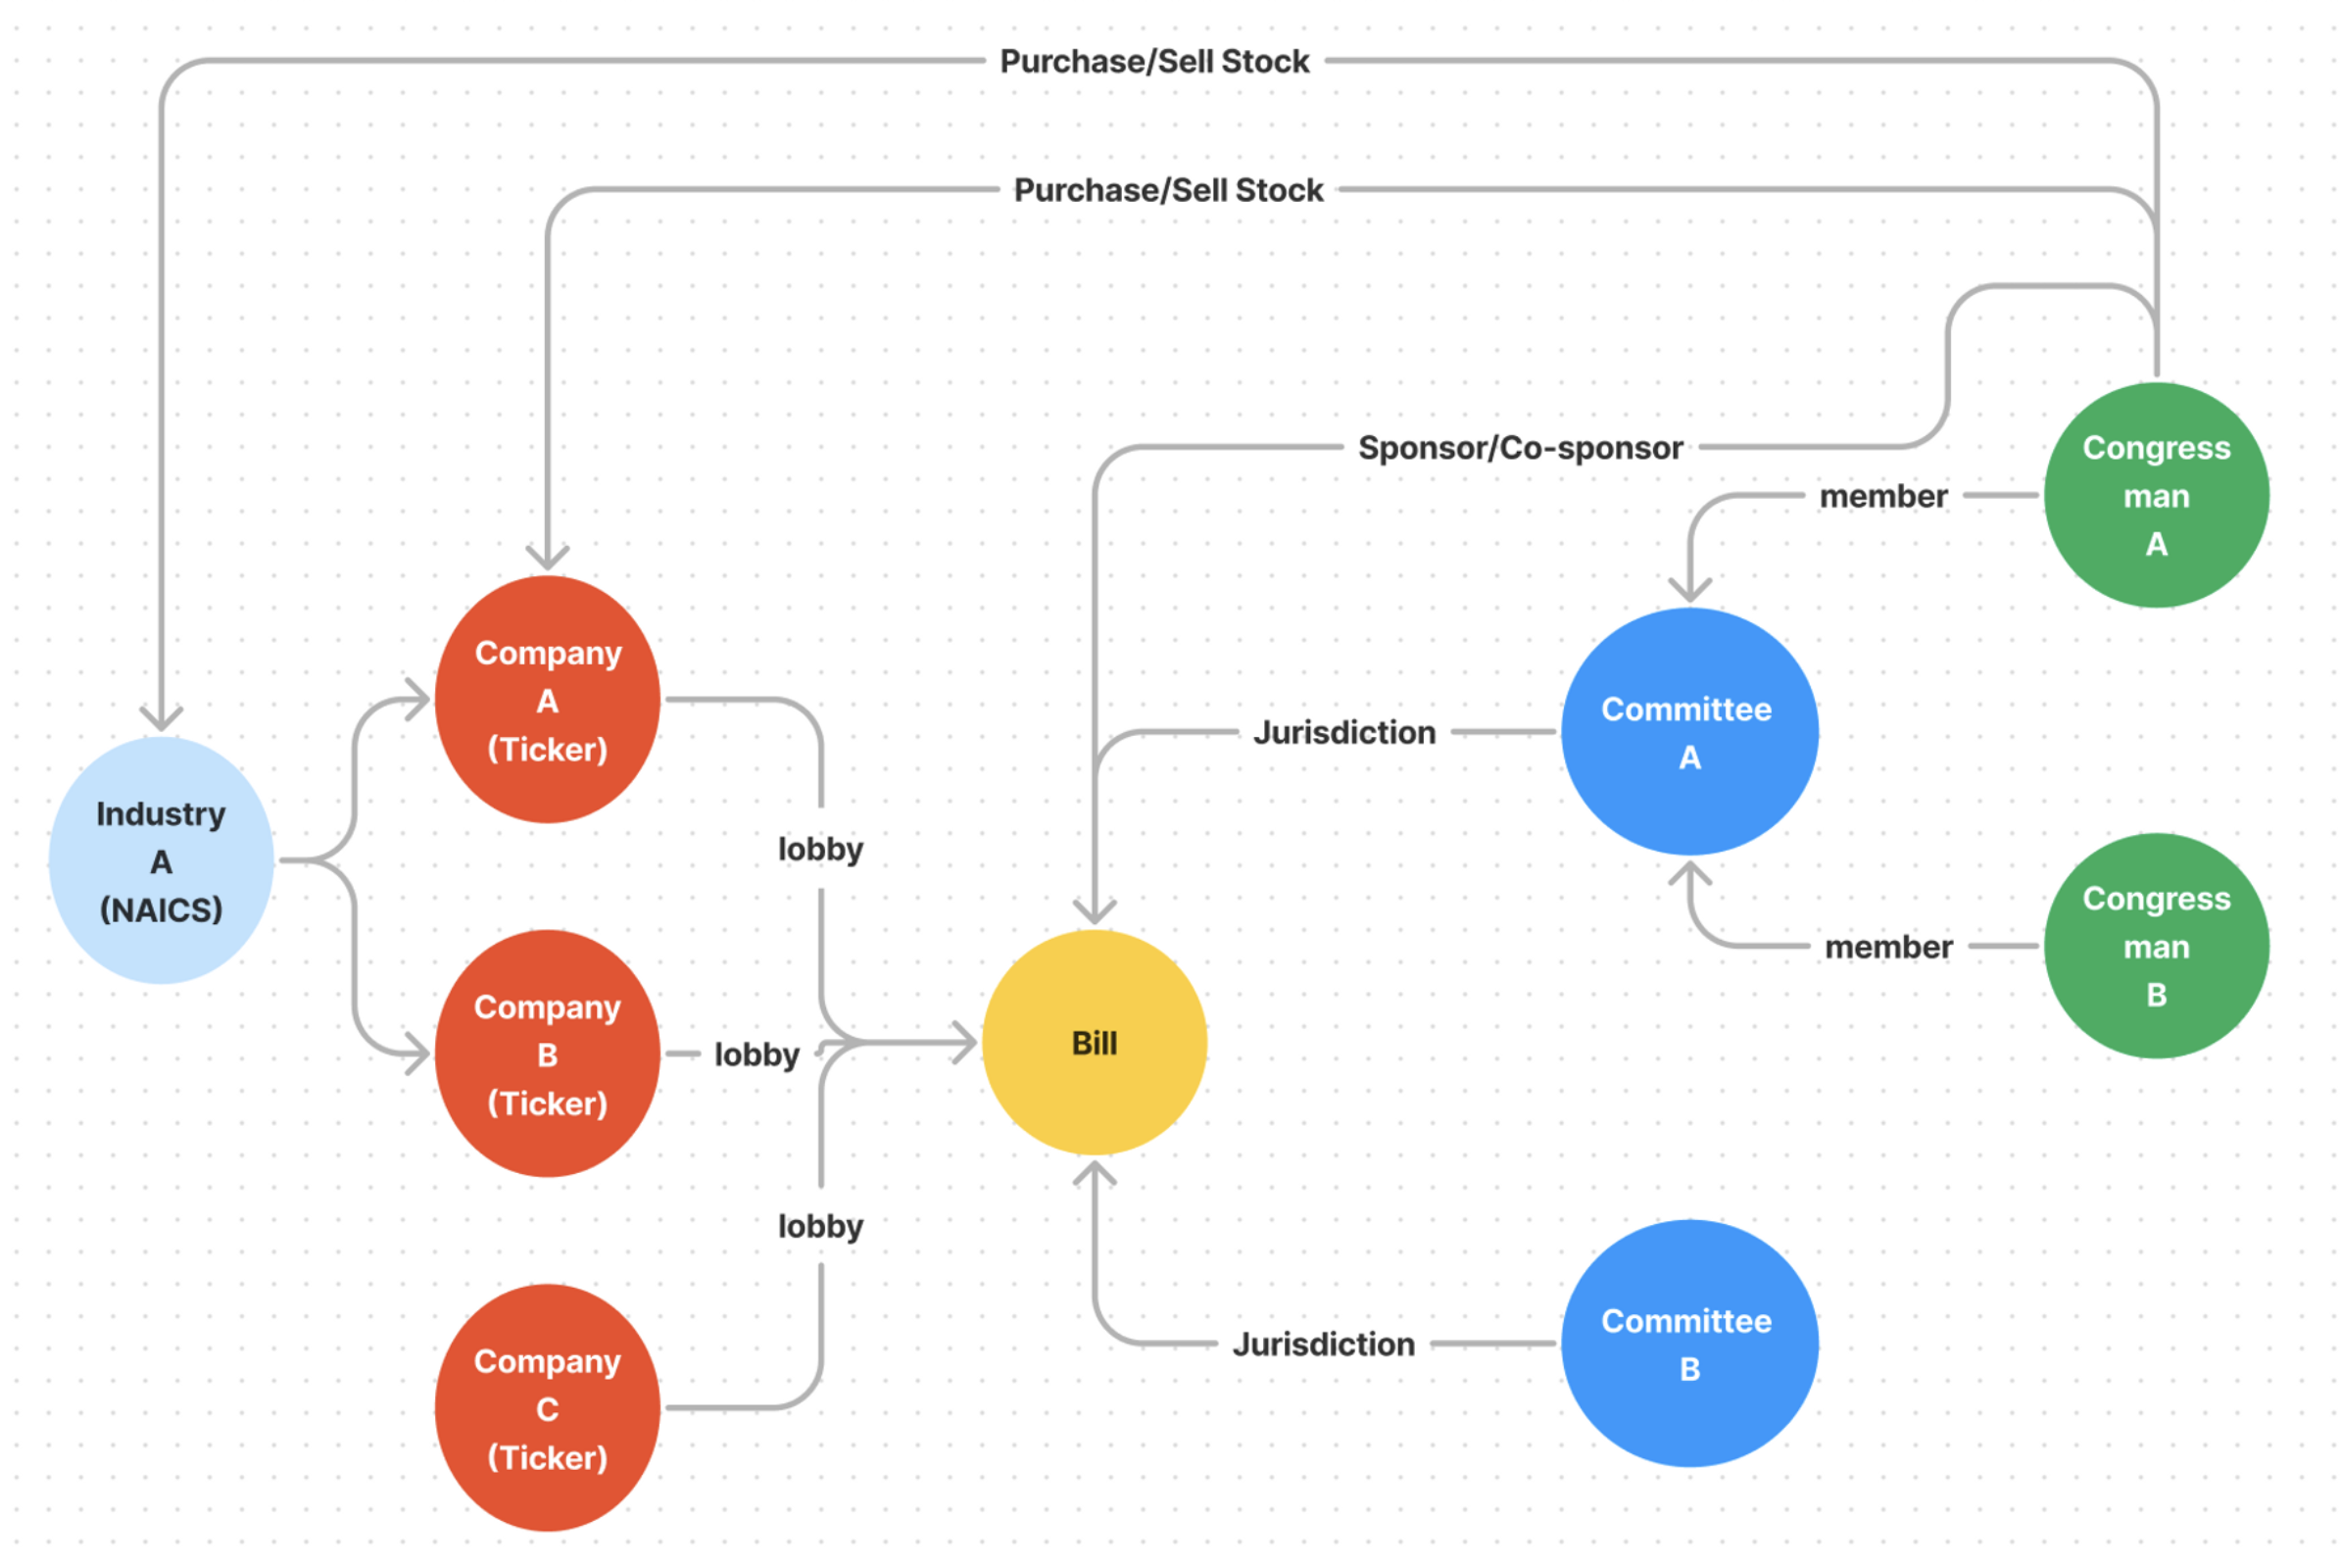
\includegraphics[width=0.75\textwidth]{imgs/graph2.png}
% %   \caption{The graph-structured data captures the congressional knowledge and includes the interactions between different types of entities.}
% %   \label{fig:graph2}
% % \end{figure}

% % \begin{figure}[h]
% %   \centering
% %   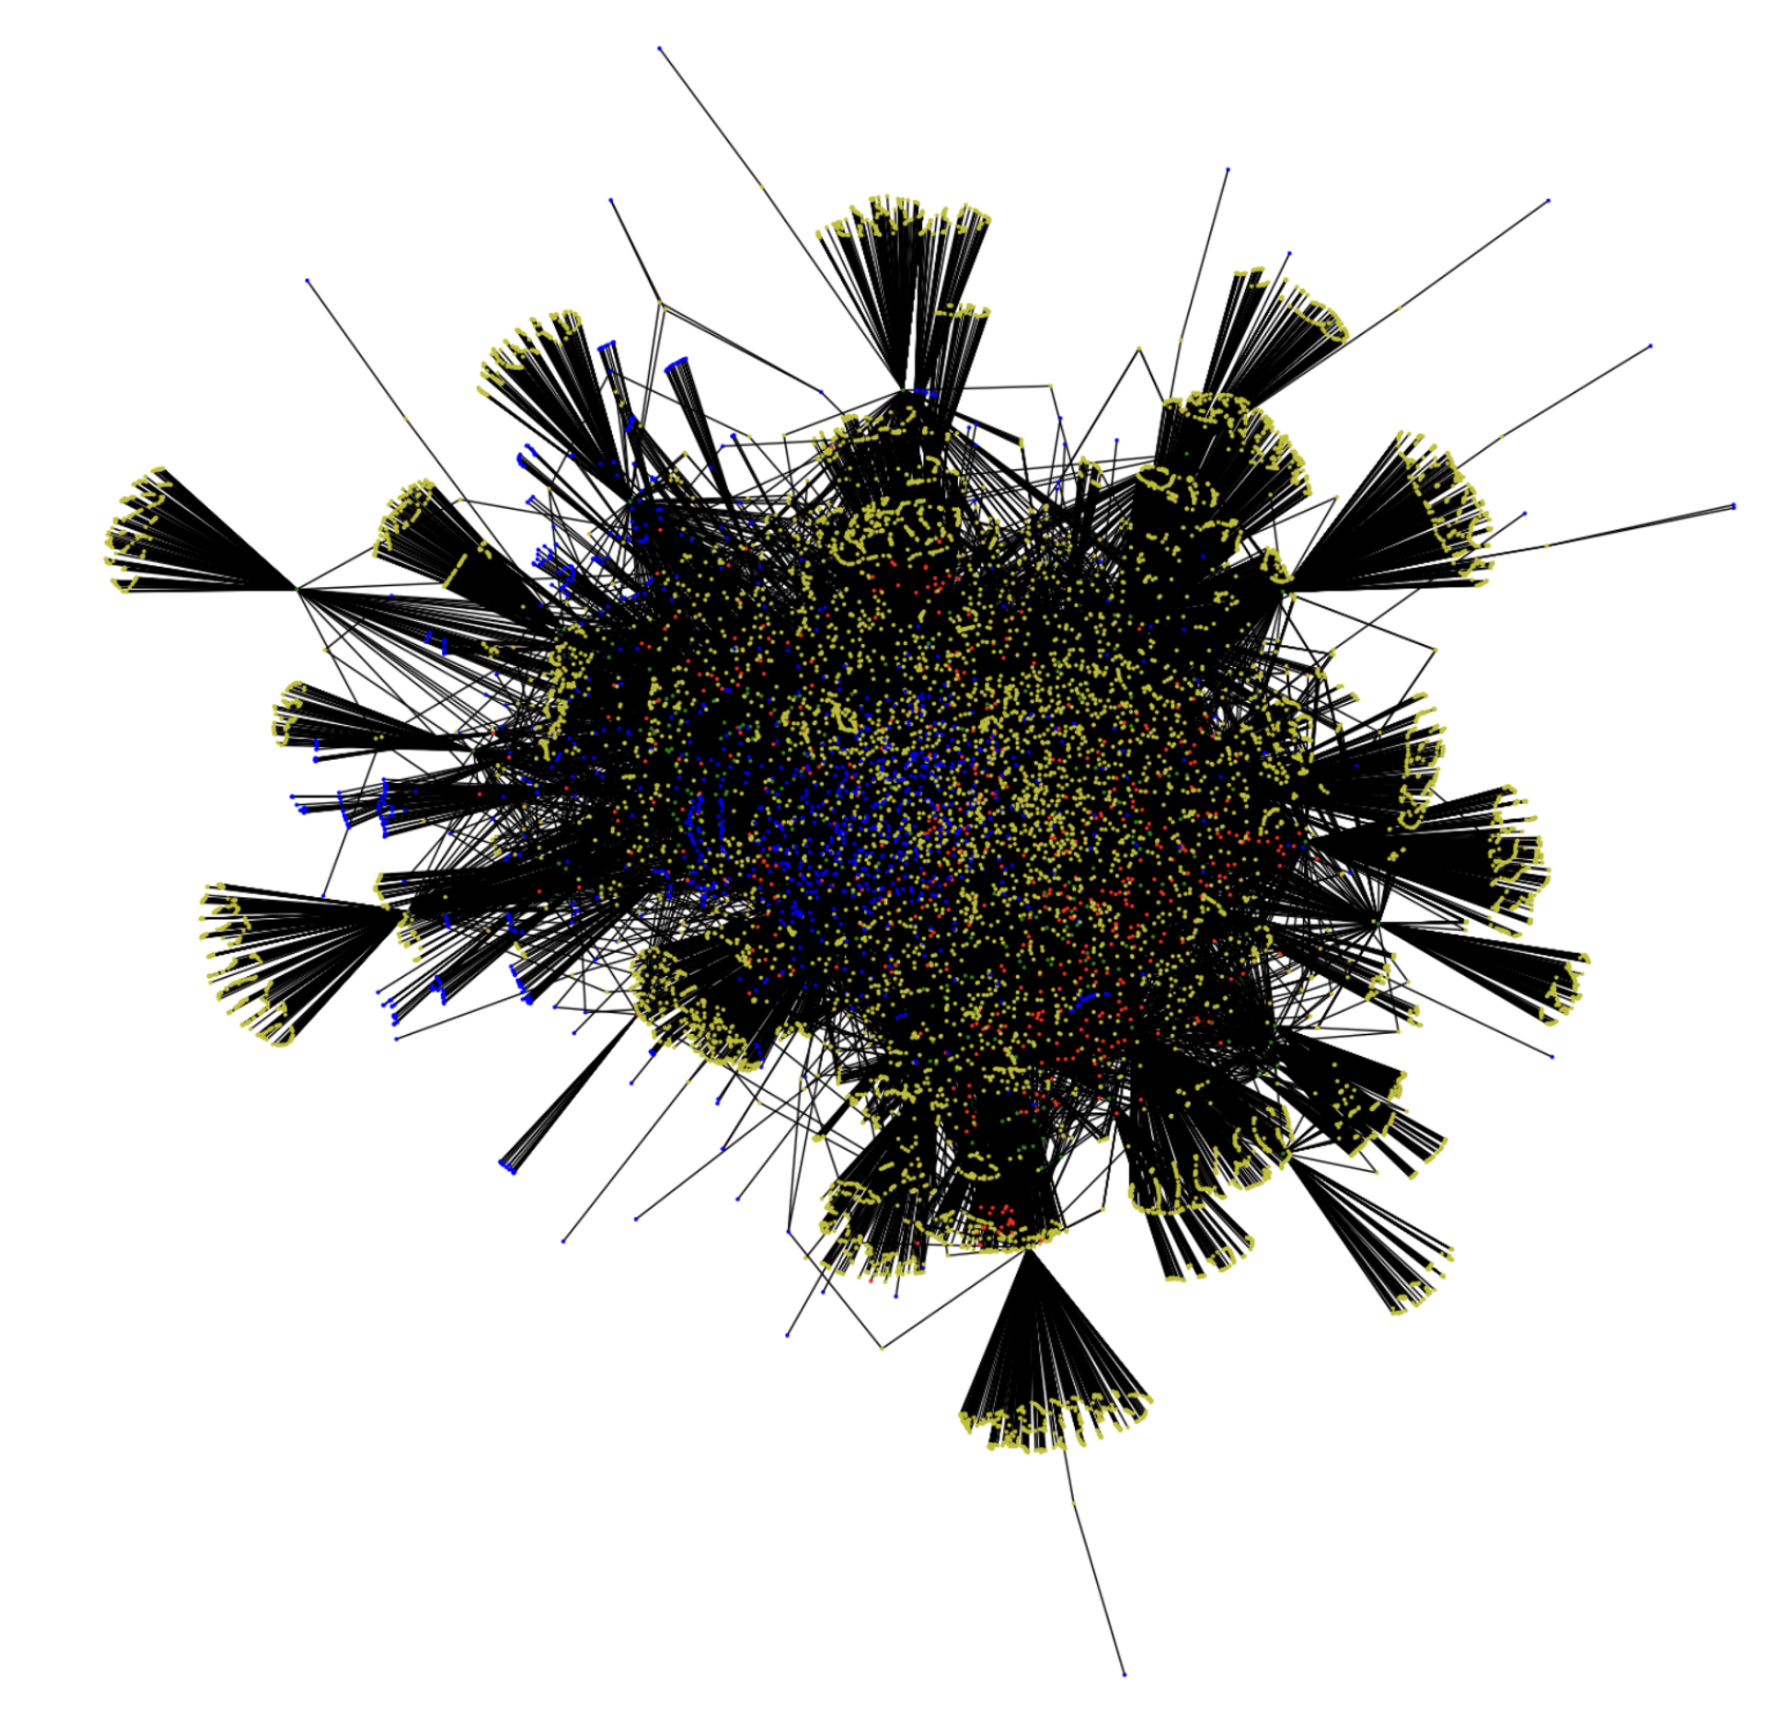
\includegraphics[width=0.75\textwidth]{imgs/graph4.png}
% %   \caption{In the graph-structured data, the yellow, blue, green, and red nodes represent bills, firms, committees, and Congressmen, respectively.}
% %   \label{fig:graph4}
% % \end{figure}


% To examine whether Congress members utilize the knowledge acquired through their positions for personal stock trading, this study estimates the causal effect of committee assignments on their stock transaction patterns. Specifically, the study investigates how being assigned to a particular committee influences the similarity between the NAICS code distribution of a Congress member's portfolio and that of the assigned committee. This is because committee assignments equip Congress members with essential expertise in specific issue areas or industries \citep{Asher1974CommitteesAT}.

% If the transaction patterns of Congress members become more similar to the industry-level information within a committee after being assigned to that committee, it would suggest that they are using their congressional knowledge for personal investment purposes.

% % As an empirical example, Figure \ref{fig:graph5} provides a diagram of Senator Ron Wyden and his NAICS code distribution of personal trading, compared with that of his assigned committee, the Senate Finance Committee (SSFI), and the Senate Banking Committee, of which he is not a member.
% % I calculated the cross-entropy between Ron Wyden's NAICS code distribution of personal trading and that of his assigned committee, the Senate Finance Committee (SSFI), which is 0.717, and that of the Senate Banking Committee (SSBK), of which he is not a member, which is 3.311. A lower cross-entropy value indicates that the two probability distributions are closer in terms of their similarity. Therefore, in Ron Wyden's case, the cross-entropy is a good measurement of the similarity between the committee and the Senator.

% % \begin{figure}[h]
% %   \centering
% %   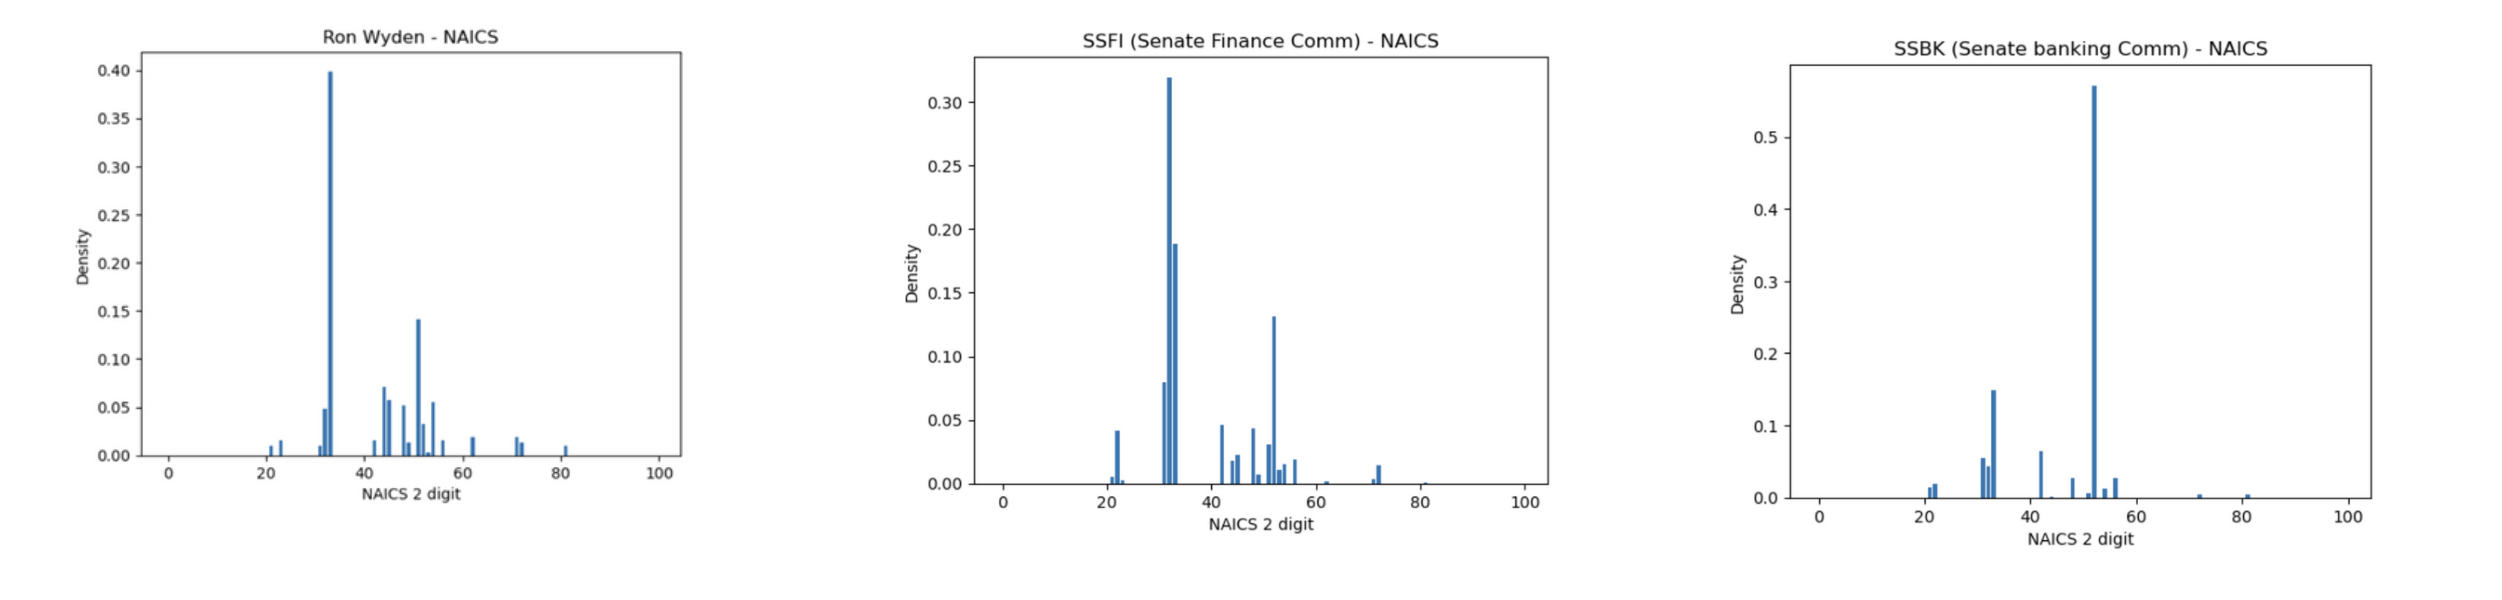
\includegraphics[width=1\textwidth]{imgs/naics.png}
% %   \caption{NAICS code distribution of Senator Ron Wyden's personal trading, compared with that of his assigned committee, the Senate Finance Committee (SSFI), and the Senate Banking Committee, of which he is not a member.}
% %   \label{fig:graph5}
% % \end{figure}


% The primary focus of this study is to estimate the conditional average treatment effect (CATE) of how a Senator's committee assignment affects the similarity between the Senator's and the assigned committee's NAICS code distribution. To estimate this, it is crucial to control for confounding variables that can influence both committee assignment and a Senator's investment behavior. The study assumes that the graph-structured data, which includes information on which firms lobby on which bills, which bills are assigned to which committees, and which Senators are members of which committees, provides all the necessary information to explain a Senator's assignment to a particular committee and their securities transactions. To support this assumption with empirical evidence, the paper will present a preliminary analysis.

% However, unlike widely used tabular data, graph-structured data cannot be directly employed to estimate a quantity of interest through a model. Since the estimation involves mathematical operations over continuous variables, graph data, being a collection of discrete objects, does not have defined operations. Nonetheless, the research emphasizes the importance of using graph-structured data, as it can encompass additional information that explains the relationships between different entities in the network during interactions in congressional activities. To overcome this computational challenge, this paper utilizes Graph Neural Networks (GNN) to learn the appropriate numerical representation specific to each Senator, who resides as a node in the graph. This representation is a numeric vector and is expected to include all the information available from the graph-structured data to explain both a Senator's stock trading behavior and their committee assignment.
% % Finally, by denoting the learned representation of Senator $i$ as $h_i = \phi_{GNN}(i, G)$, the study can estimate the conditional average treatment effect (CATE) by learning estimators for both $\mu_0(h_i) \equiv \mathbb{E}\left[Y_i \mid H=h_i, T_i=0\right]$ and $\mu_1(h_i) \equiv \mathbb{E}\left[Y_i \mid H=h_i, T_i=1\right]$, and using the formula $\text{CATE}(h_i) = \mu_1(h_i) - \mu_0(h_i)$. This allows the study to estimate the effect of committee assignment on the similarity between a Senator's and the assigned committee's NAICS code distribution, while controlling for potential confounders through the learned representation $h_i$.
% % For the estimator of $\mu_0(h_i)$ and $\mu_1(h_i)$, the study will use the Treatment Agnostic Regression Network (TARNet) \citep{tarnet}, which extends T-learners \citep{tlearner} with additional layers of neural networks that learn a shared representation of $h_i = \phi_{GNN}(i, G)$ for the treatment and control groups in a balanced way. By doing so, the neural network can effectively perform its regression task to estimate CATE, even though $h_i$ is asymmetrically distributed between the treatment and control groups.

% There are a total of 62 different committees, and CATE is estimated for each committee separately. By evaluating these CATE values, the paper aims to quantitatively evaluate how committee assignment heterogeneously affects Senators' behavior across committees and among Senators themselves.
% % In addition, it is necessary to control for the confounders to estimate the effect correctly. I assume that the graph-structured data, which includes interactions between firms, bills, committees, and congressmen, and their stock transactions includes all possible confounders that affect committee assignments and their impact on the dependent variable, which is the industry-level similarity between the committee and the congressmen's portfolio. However, in terms of methodology, the question remains about how to control graph-structured data to estimate the treatment effect. Unlike tabular data with numeric values in each item, graph-structured data is a discrete object and thus cannot be computed in typical models.
% % However, thanks to recent developments in representational learning and neural networks, a specific architecture of neural network (called a ``Graph Neural Network'') can learn a good numeric representation of each node by considering its connection with its neighboring nodes in the graph.

% % To determine what constitutes a ``good'' representation of graph-structured data, one can evaluate whether the representation performs the downstream task effectively, which in this case is estimating CATE. The Graph Neural Network learns a representation, denoted as $\phi_{GNN}(X)$, for a given graph-structured data $X$, and I use $\phi_{GNN}(X)$ to estimate the effect of committee assignments on the dependent variable. However, because $\phi_{GNN}(X)$ will be a highly non-interpretable covariate that encodes complex interactions included in the graph, I use meta-learners \citep{metalearner} to estimate CATE using $\phi(X)$. Meta-learners are a family of estimators that combine supervised learning, also known as ``base-learners'', in a specific way while allowing the base learners to take any form, including neural networks. 
% % In this case, I use the Treatment Agnostic Regression Network (TARNet) \citep{tarnet}, which extends T-learners \citep{tlearner}, which is a variant of meta-learners, with additional layers of neural networks that learn a shared representation of $\phi(X)$ for the treatment and control groups in a balanced way. By doing so, the neural network can effectively perform its regression task to estimate CATE, even though $\phi(X)$ is complex, while jointly learning the balanced representation of $\phi(X)$.


% The paper aims to make two main contributions. Firstly, it substantively proves the existence of insider trading by explicitly showing that committee membership changes affect Congressmen's investment behavior to become similar to the information available from the committee. Secondly, it demonstrates a novel methodological approach to estimate causal quantities using graph-structured data by leveraging representation learning via Graph Neural Network. Therefore, the paper proposes a model and learning scheme that combines a Graph Neural Network and meta-learners to learn CATE, conditioning on the output of the Graph Neural Network. 
% % However, the common limitation of these studies is that they do not specify the exact source of congressional knowledge and how that knowledge influences their investment behavior.

% % Although many studies have investigated the investment behavior of congressmen, there are still gaps in the literature. \cite{zi11} and \cite{zi24} found that Senators and House representatives beat the market and enjoy excess returns while \cite{eg13} found that they don't. 
% % However, the common limitation of current work is that they don't specify the exact source of congressional knowledge and how that knowledge affects their behavior.

% % The biggest problem in this line of research is about how to prove they ``do'' invest with which ``privileged knowledge''.
% % The main issue in this area of research is how to prove that politicians are using their inside knowledge to make investments. Just because they make a lot of money from their investments doesn't necessarily mean they are using privileged information. However, many high-profile cases have linked this knowledge to their committee assignments, sponsoring of bills, or their home state and potential connections to local businesses. Therefore, future research should focus on developing a reliable method to track down the sources of this privileged knowledge that is more closely linked to investments that show abnormally high returns. This will help to identify which politicians are involved in unethical financial practices and how they are doing it.


% % In my initial research, I analyzed the excess return for each transaction made by Senators with specific stocks, comparing the return on investment to the federal reserve rates. The results, shown in Figure \ref{fig:agg-ex-r}, suggest that Senators do not generally make significant excess returns from their trading, which is consistent with the findings of \cite{eg13}. However, I did find a few outliers who made substantial gains, some of which have been reported by journalists, while others have not been publicly exposed. An important finding from these outliers is that committee information seems to enable some Senators to enjoy unusually high returns from their trading. 
% % For instance, Senator Ron Wyden from Oregon traded three semiconductor industry stocks, namely AMAT, KLAC, and AVGO, and gained a significant excess return of 170\%, 115\%, and 70\%, respectively (refer to Figure \ref{fig:agg-ex-r}). What stands out is that he bought all three stocks on the same day, April 6, 2020, during a time when the market was falling due to concerns about the pandemic's impact on the economy. He then sold all three stocks on the same day, April 6, 2021, after President Biden proposed a \$50 billion boost to the US chips industry. It is reasonable to assume that Senator Ron Wyden, being the chair of the Senate finance committee, had prior knowledge of this issue before it was made public. This is because the Senate finance committee introduced the bill ``S.3933 - CHIPS for America Act'' after the announcement on June 10, 2020.

% % As another example, Senator Ron Wyden made a 38\% ROI from his investment in an American wine producing company (Constellation Brand, Inc. - Ticker: STZ) when the Trump administration imposed additional tariffs on wines imported from Europe.
% % Since the Senate finance committee has jurisdiction over trade, it is reasonable to assume that Senator Ron Wyden had prior knowledge of this issue before it was made public.

% % In addition, David Perdue, a former senator from Georgia, obtained an estimated excess return of 10\% from his investment in BWX Technologies Inc., a company that supplies nuclear components to the US Navy. What is notable is that he made consecutive purchases of the stock that turned into sales after he was named chairman of the Senate Armed Services Subcommittee on Seapower.

% % \begin{figure}[h]
% %   \centering
% %   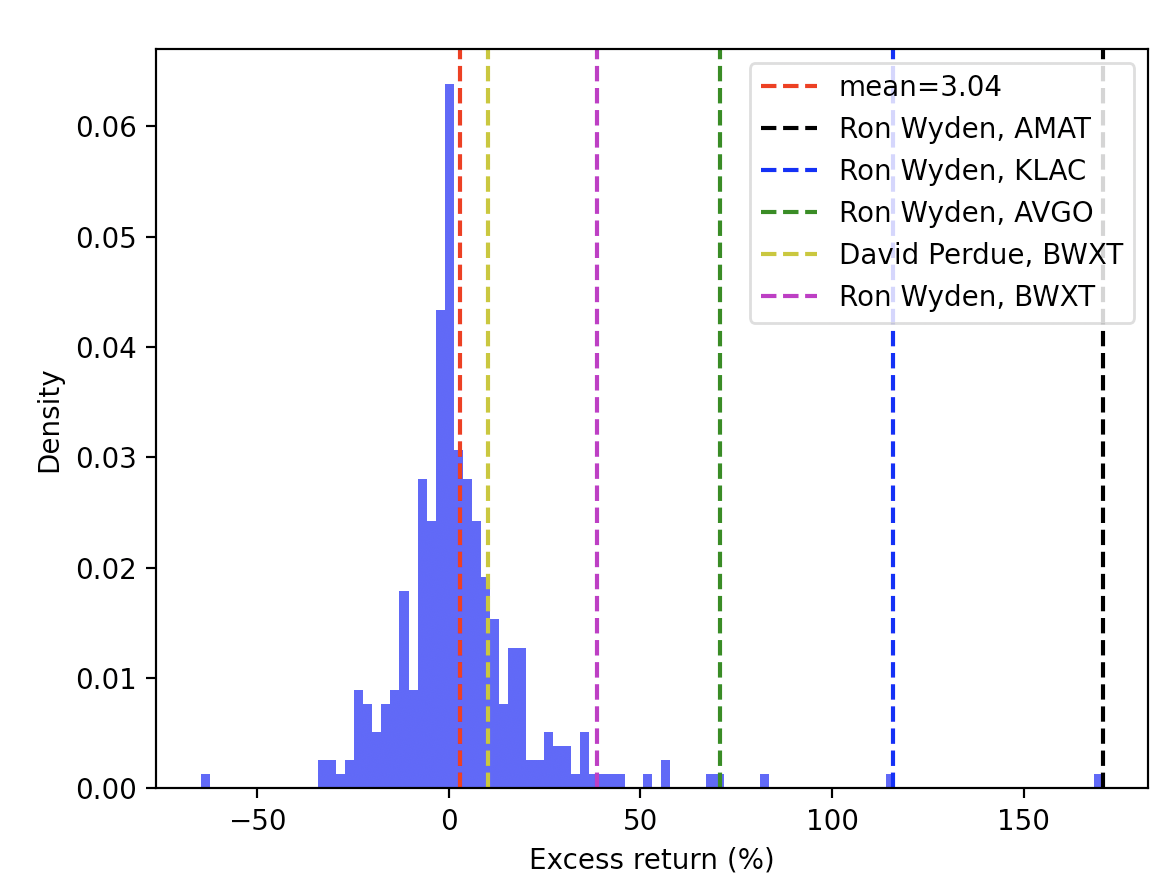
\includegraphics[width=1\textwidth]{imgs/ex-r/aggregate.png}
% %   \caption{Distribution of mean of each distribution of excess return for $333$ distinct pairs of (Senator, Ticker).}
% %   \label{fig:agg-ex-r}
% % \end{figure}

% % \begin{figure}[h]
% %   \centering
% %   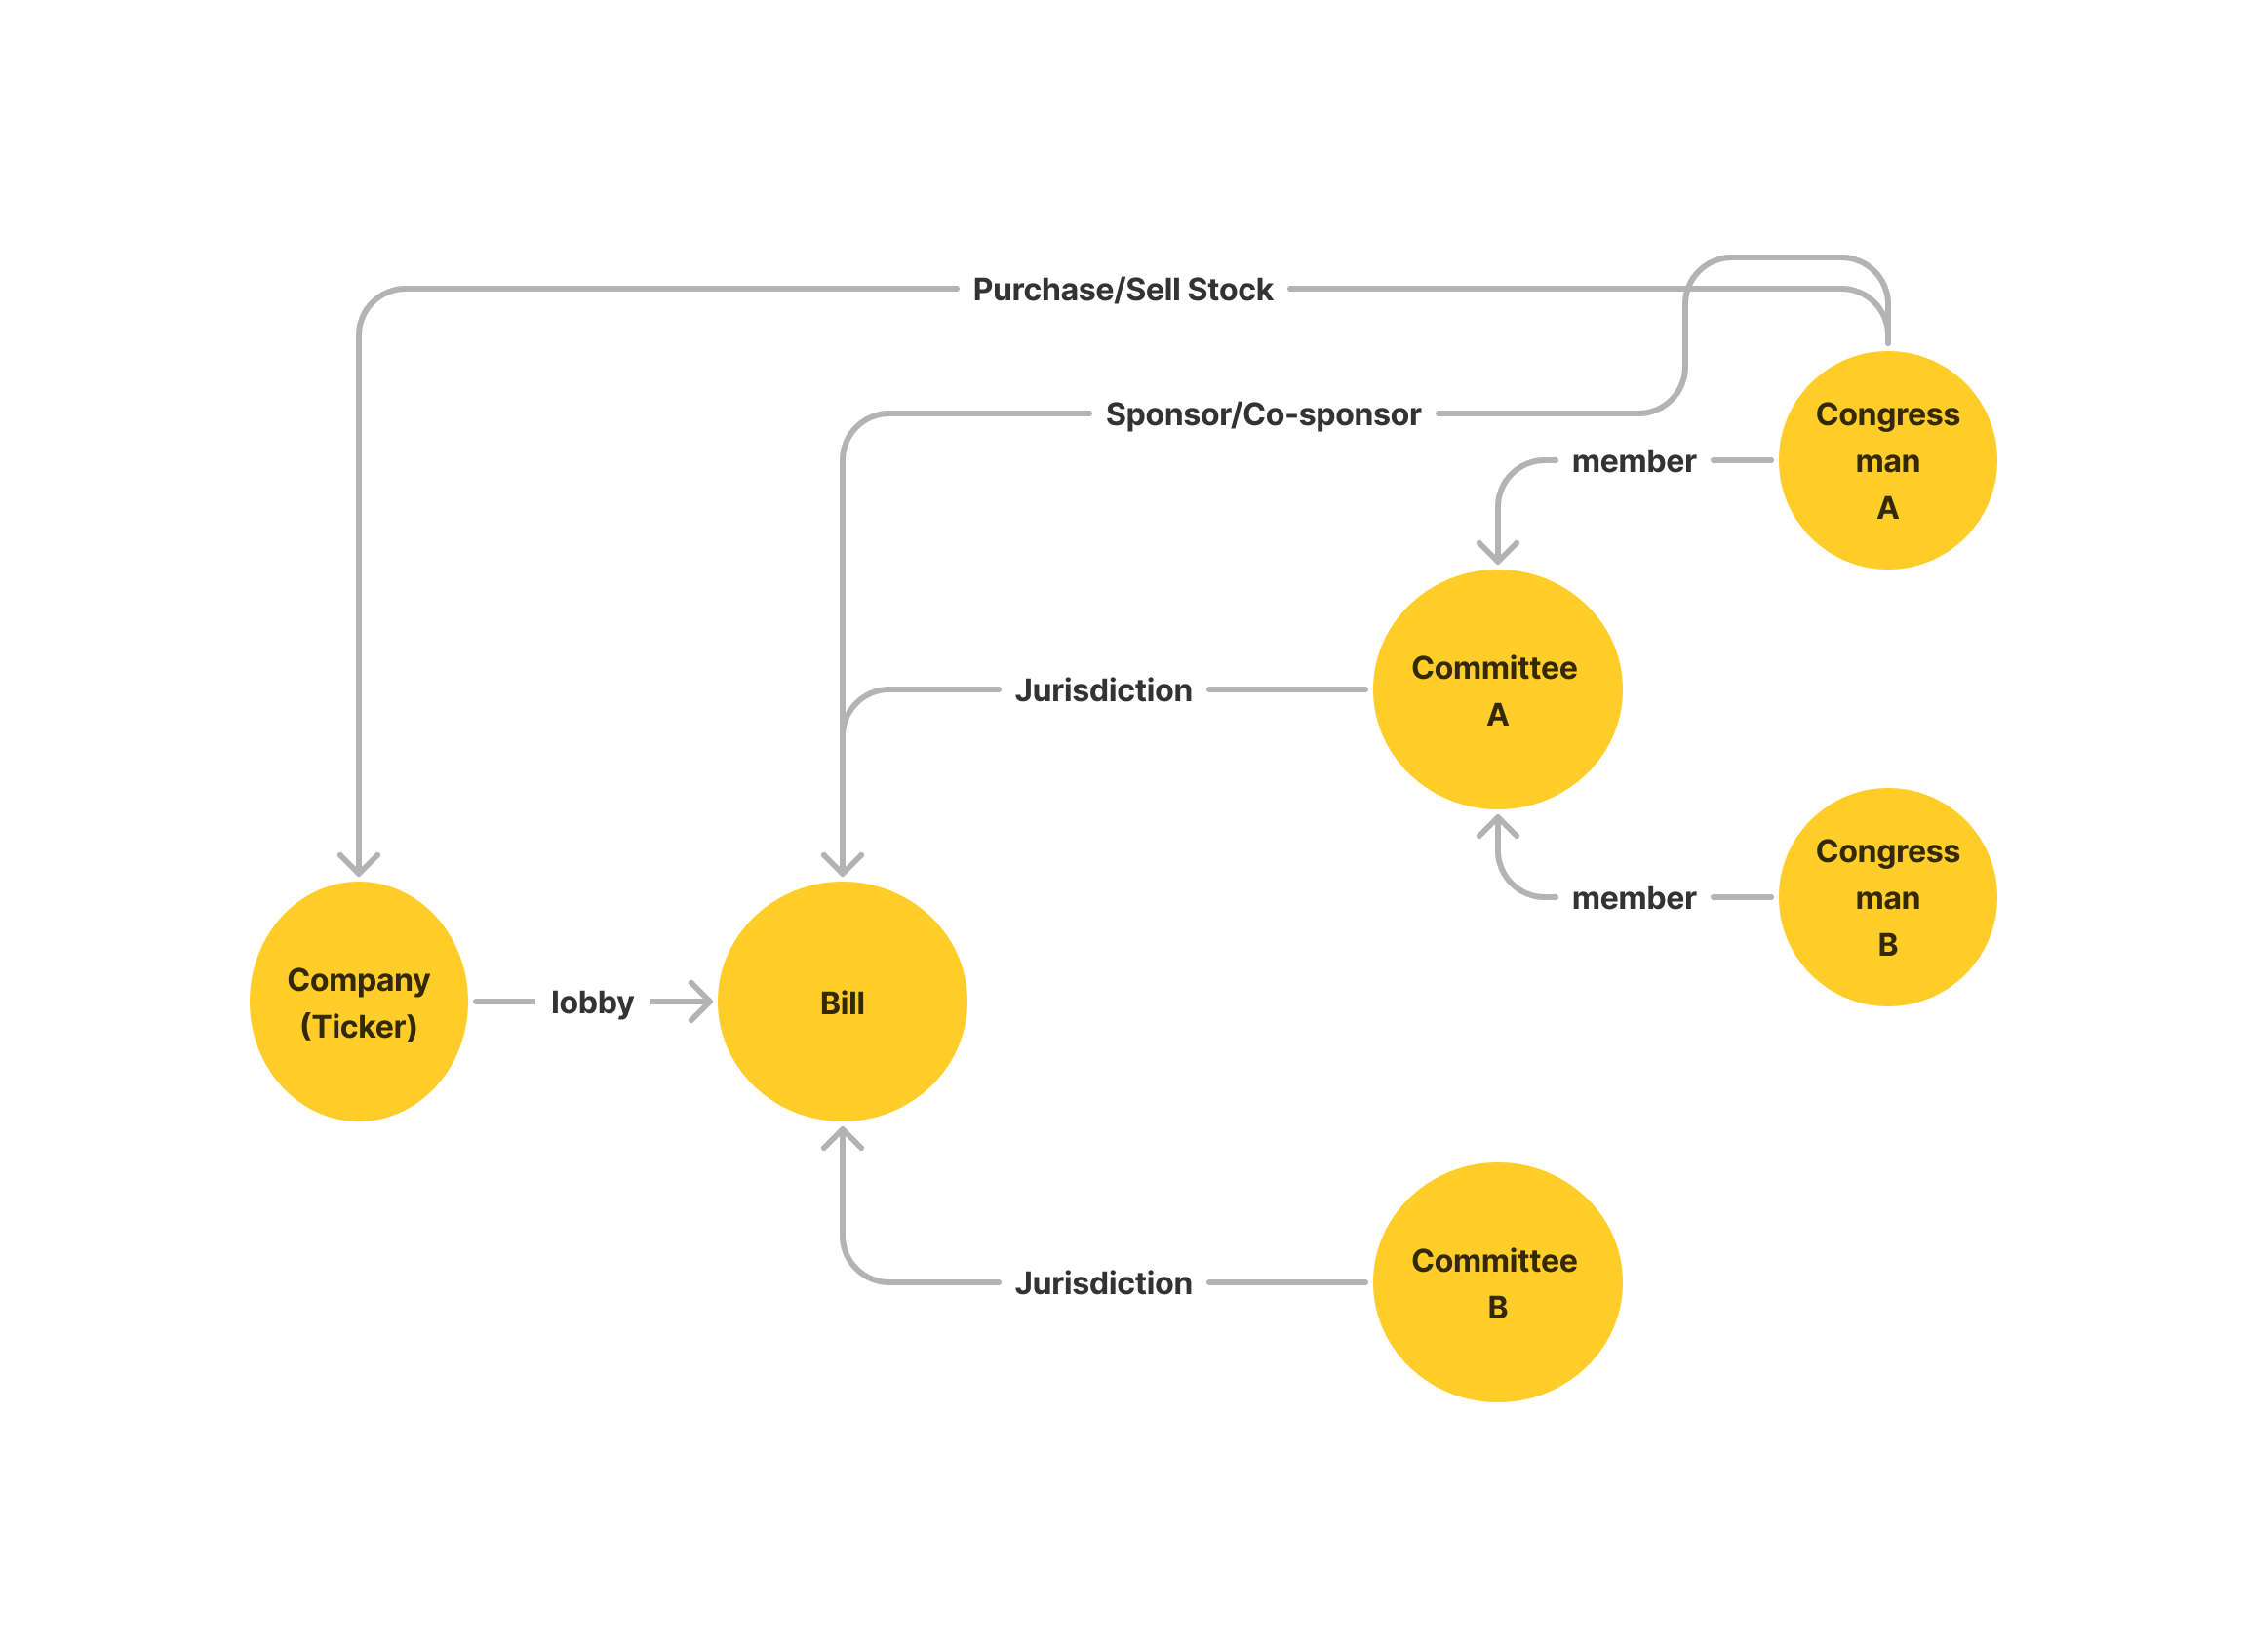
\includegraphics[width=1\textwidth]{imgs/cgd.png}
% %   \caption{Interaction graph between committees, bills, companies, and congressmen in congressional investment.}
% %   \label{fig:cbd}
% % \end{figure}


\section{Data} \label{data}

\subsection{Data Description}
% The data utilized in this study is a congressional network that records the legislative activities of Senators and their investment behavior. The network is created by merging data from LobbyView with Senate financial disclosures. It contains details about the Senators' buying/selling of company stocks, the dates of these transactions, their committee assignments during specific Congresses, the bills that are being lobbied by companies, and which bills are assigned to which committee. The firms are classified according to NAICS codes, as shown in Figure 
The data utilized in this study is a large graph-structured dataset that captures both congressional activities and Congresspersons' stock transactions simultaneously. The dataset, represented as a heterograph, consists of various types of nodes and edges that incorporate transaction data, detailing Senate and House members' stock buying and selling activities, along with the specific dates of those transactions. The graph-structured data also encompasses information on congressional activities, such as committee assignments, bills being lobbied by firms, bill assignments to committees, and firms classified under specific NAICS codes. The detailed specifications of the node types can be found in Table \ref{tab:nodes}, while the edge types are described in Table \ref{tab:edges}, encompassing the connections between firms and their respective NAICS codes.
Different types of nodes and their relationships, captured by different types of edges, are illustrated in Figure \ref{fig:cbd}.
\begin{table}[h!]
  \centering
  \caption{Heterograph (Nodes)}
  \label{tab:nodes}
  \begin{tabular}{@{}llll@{}}
  \toprule
  Node Type & N & Period & Source \\ \midrule
  Firm (Ticker) & 4,202 & - & Lobbyview \& Finance Disclosure \\
  Bills & 47,767 & 110-117th Congress & Lobbyview \\
  Congressperson & 2,431 & 113-118th Congress & Lobbyview \& Finance Disclosure \\
  Committee & 556 & - & Lobbyview \\
  NAICS code & 744 & - &  naics.com \\ \bottomrule
  \end{tabular}
\end{table}

\begin{table}[h!]
  \centering
  \caption{Heterograph (Edges)}
  \label{tab:edges}
  \begin{tabular}{@{}llll@{}}
  \toprule
  Edge Types & N & Period & Source \\ \midrule
  Congressperson- Buy/Sell- Firm (Ticker) & 24,675 & [2013-01-24, 2023-03-08] & Finance Disclosure \\
  Firm (Ticker) - Lobby On - Bill & 148,487 & [2016-01-02, 2022-02-24] & Lobbyview \\
  Ticker- Classified as - NAICS Codes & 4,147 & - & Finance Disclosure \& naics.com \\
  Bill- Referred to - Committee & 75,626 & [2016-01-05, 2021-12-17] & Lobbyview \\
  Congressperson- Assigend to - Committee & 11,698 & 115-117th Congress & Finance Disclosure \& Lobbyview \\ 
  \bottomrule
  \end{tabular}
  \end{table}

\begin{figure}[h!]
  \centering
  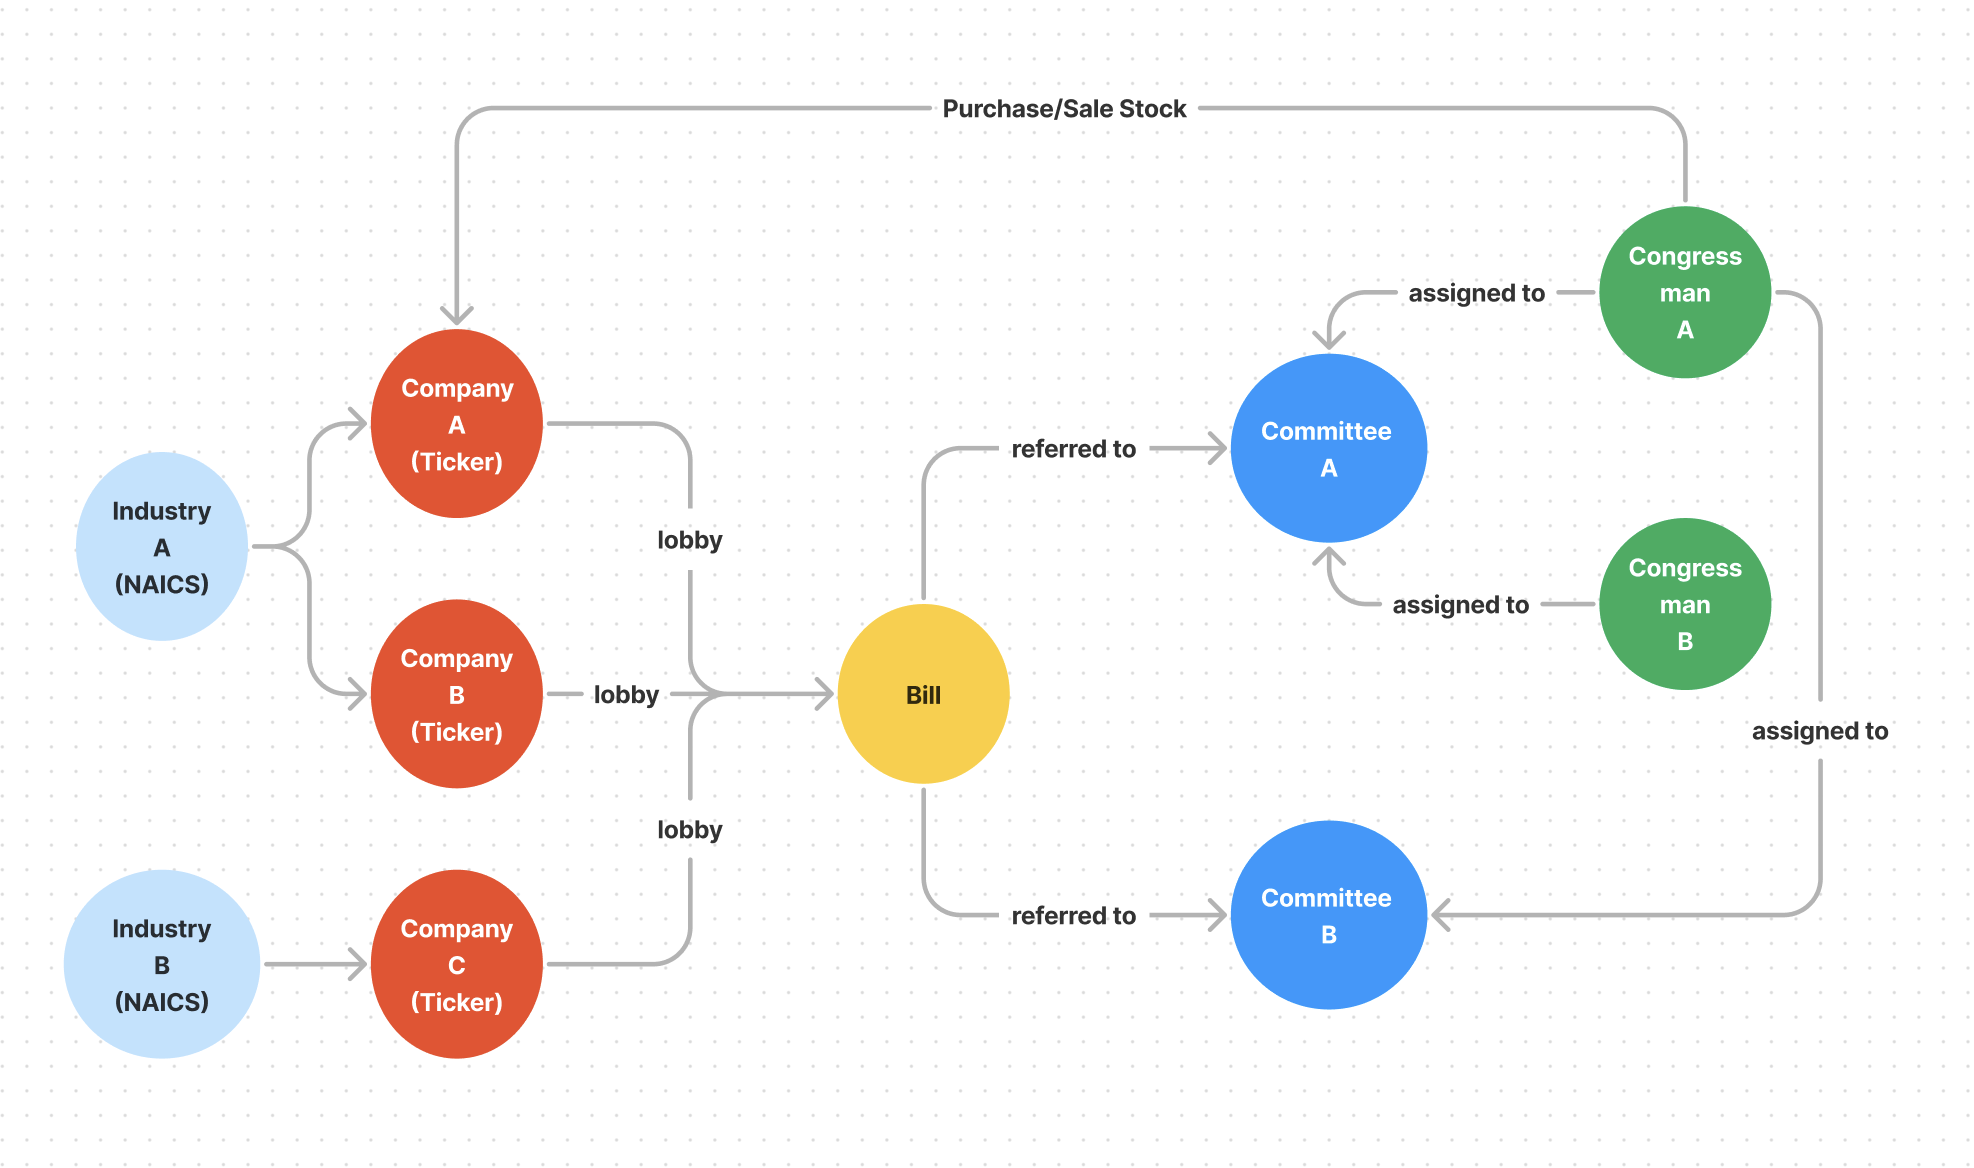
\includegraphics[width=1.0\textwidth]{imgs/illus.png}
  \caption{The network data includes various types of nodes and edges that represent different entities and interactions within the congressional activities and investment behavior of Congresspersons.}
  \label{fig:cbd}
\end{figure}

To provide a more concrete understanding of the data, Figure \ref{fig:trip} displays a subgraph related to Senator Ron Wyden's transaction in Trip Advisor stock (Ticker: TRIP). 
This subgraph illustrates the relationships between Senator Ron Wyden's congressional activities, including his membership in the Senate Finance Committee, his involvement with a specific bill related to airport improvements, and the economic sectors represented by NAICS codes, thereby providing insights into how these activities could potentially influence or be influenced by his stock transactions.

\begin{figure}[h]
  \centering
  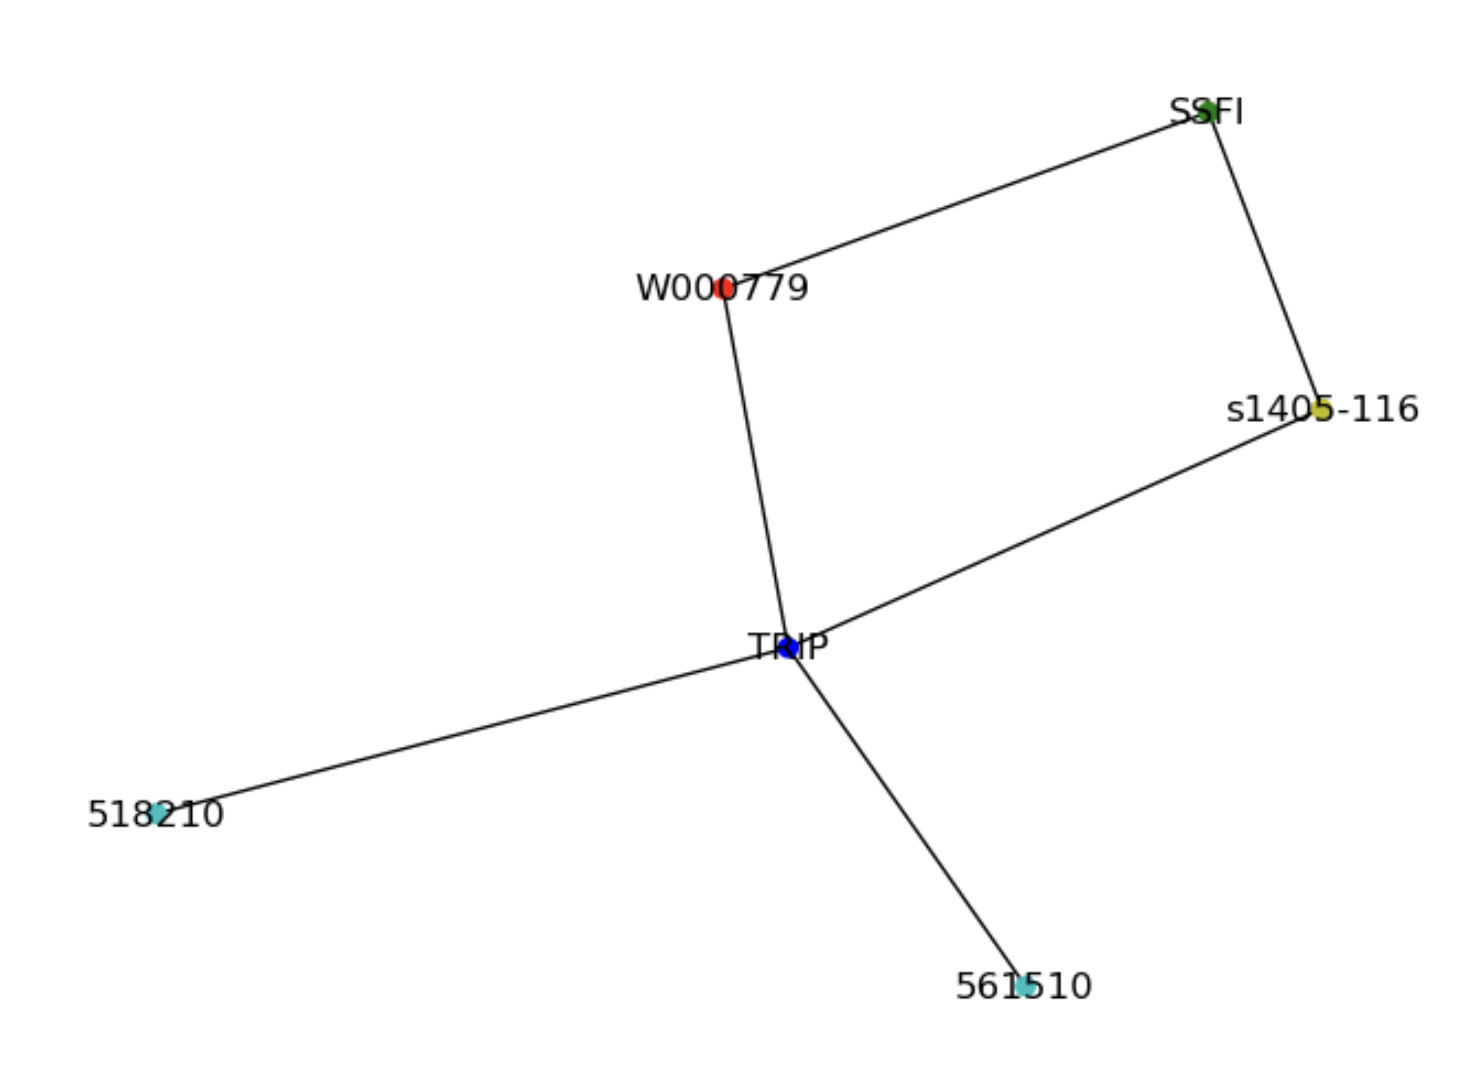
\includegraphics[width=1\textwidth]{imgs/trip.png}
  \caption{\textbf{A subgraph illustrating the congressional network related to the transaction of Senator Ron Wyden's Trip Advisor stock.} The node labeled W000779 corresponds to Ron Wyden's bioguide-id, which is a unique identifier provided by Congress for each senator. SSFI represents the Senate Finance Committee, of which Ron Wyden is a member. S1405-116 is a bill in the 116th Congress that revises requirements for the airport improvement program and pilot program for passenger facility charges at nonhub airports. The node labeled 518210 represents the NAICS Code for Data Processing, Hosting, and Related Services, while 561510 represents Travel Agencies.}
  \label{fig:trip}
\end{figure}

In addition to the subgraph related to Senator Wyden's transactions, I also provide two more subgraphs in Figure \ref{fig:semi} and Figure \ref{fig:ssbk} to further aid understanding. These figures capture the industry-level congressional activities, illustrating how firms project their interests through lobbying to specific bills, and how committees oversee such bills. These subgraphs collectively demonstrate how firm/industry-level specific interests are funneled through lobbying to bills and aggregated to specific committees, ultimately conveying this information to congresspersons assigned to those committees. By examining these interconnections, we can gain a deeper understanding of the potential influences on stock transactions made by members of Congress.

\begin{figure}[h!]
  \centering
  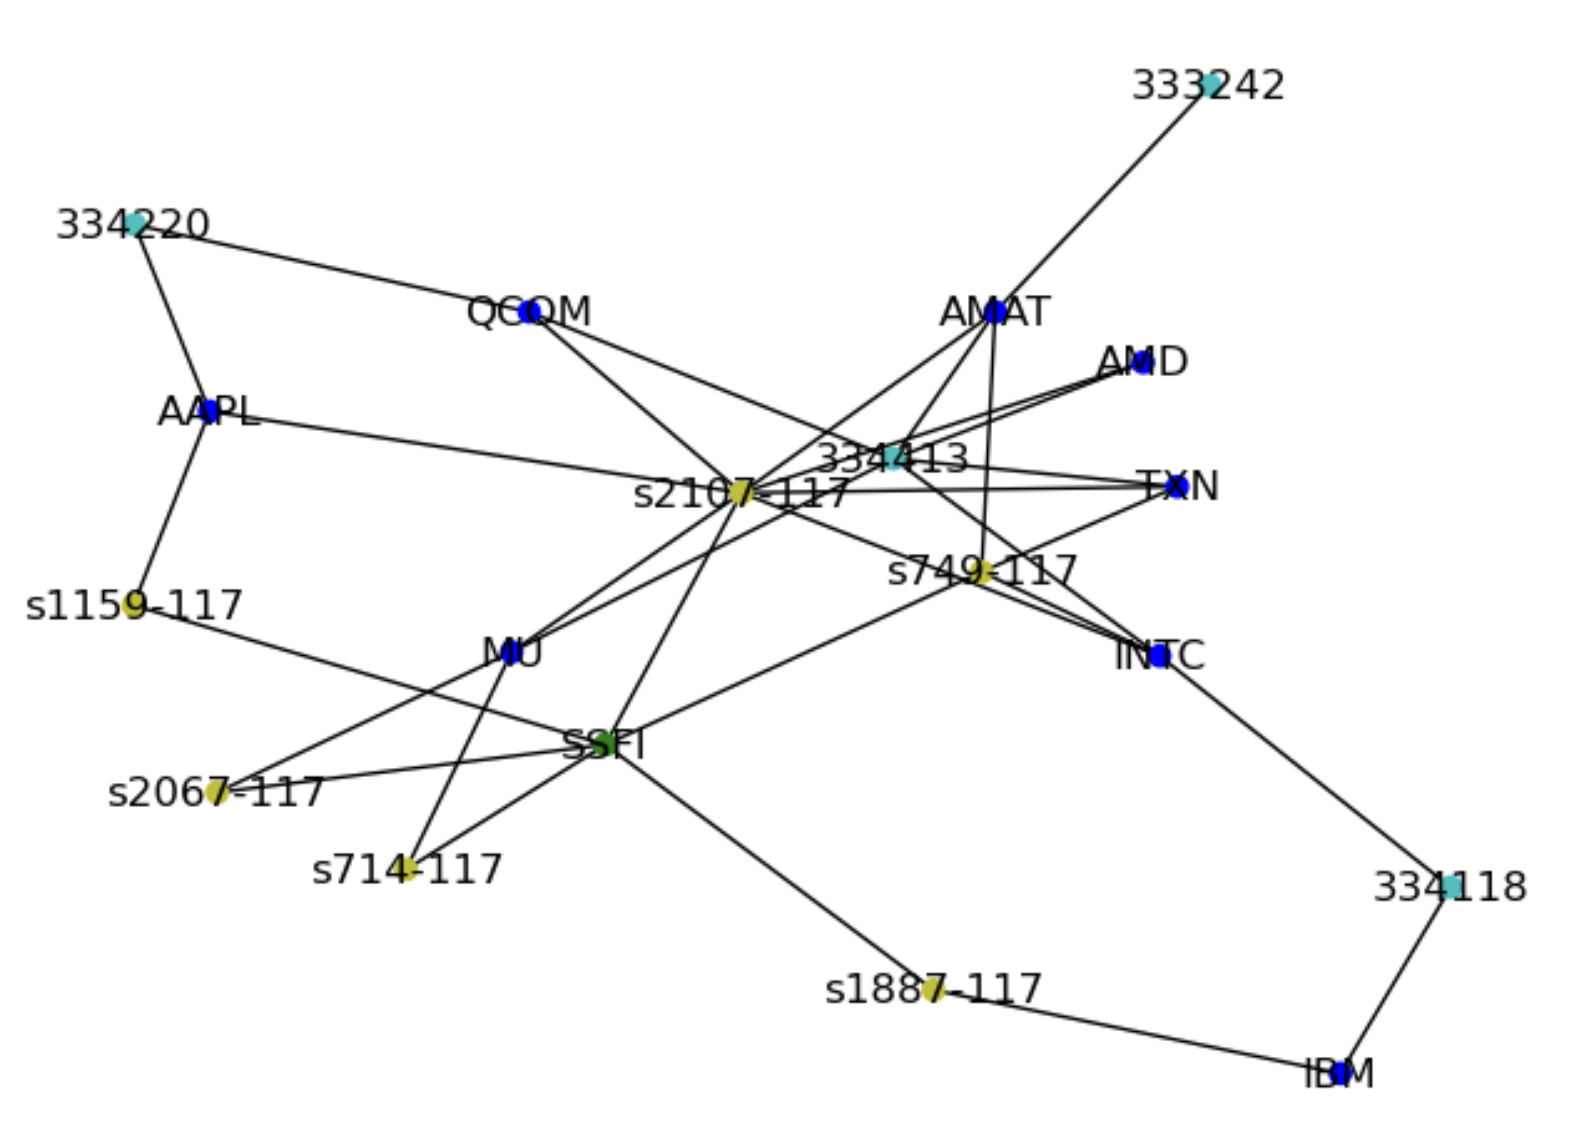
\includegraphics[width=1\textwidth]{imgs/semic.png}
  \caption{\textbf{Subgraph capturing how the semiconductor industry's interests were funneled through the Senate Finance Committee during the 117th Congress} The NAICS code 334413 indicates Semiconductor and Related Device Manufacturing, which involves companies such as Qualcomm (QCOM), Intel (INTC), and Advanced Micro Devices (AMD), lobbying for bills such as the CHIPS Act and FABS Act that are closely related to the subsidization of semiconductor manufacturing facilities. Relevant companies such as Apple Inc. and IBM, with NAICS codes of 334220 Wireless Communications Equipment Manufacturing and 334118 Computer Equipment Manufacturing, respectively, are direct customers of these semiconductor chips for manufacturing smartphone and computer hardware. The bills in which these companies have an interest are assigned to the Senate Finance Committee as well.
  }
  \label{fig:semi}
\end{figure}

\begin{figure}[h!]
  \centering
  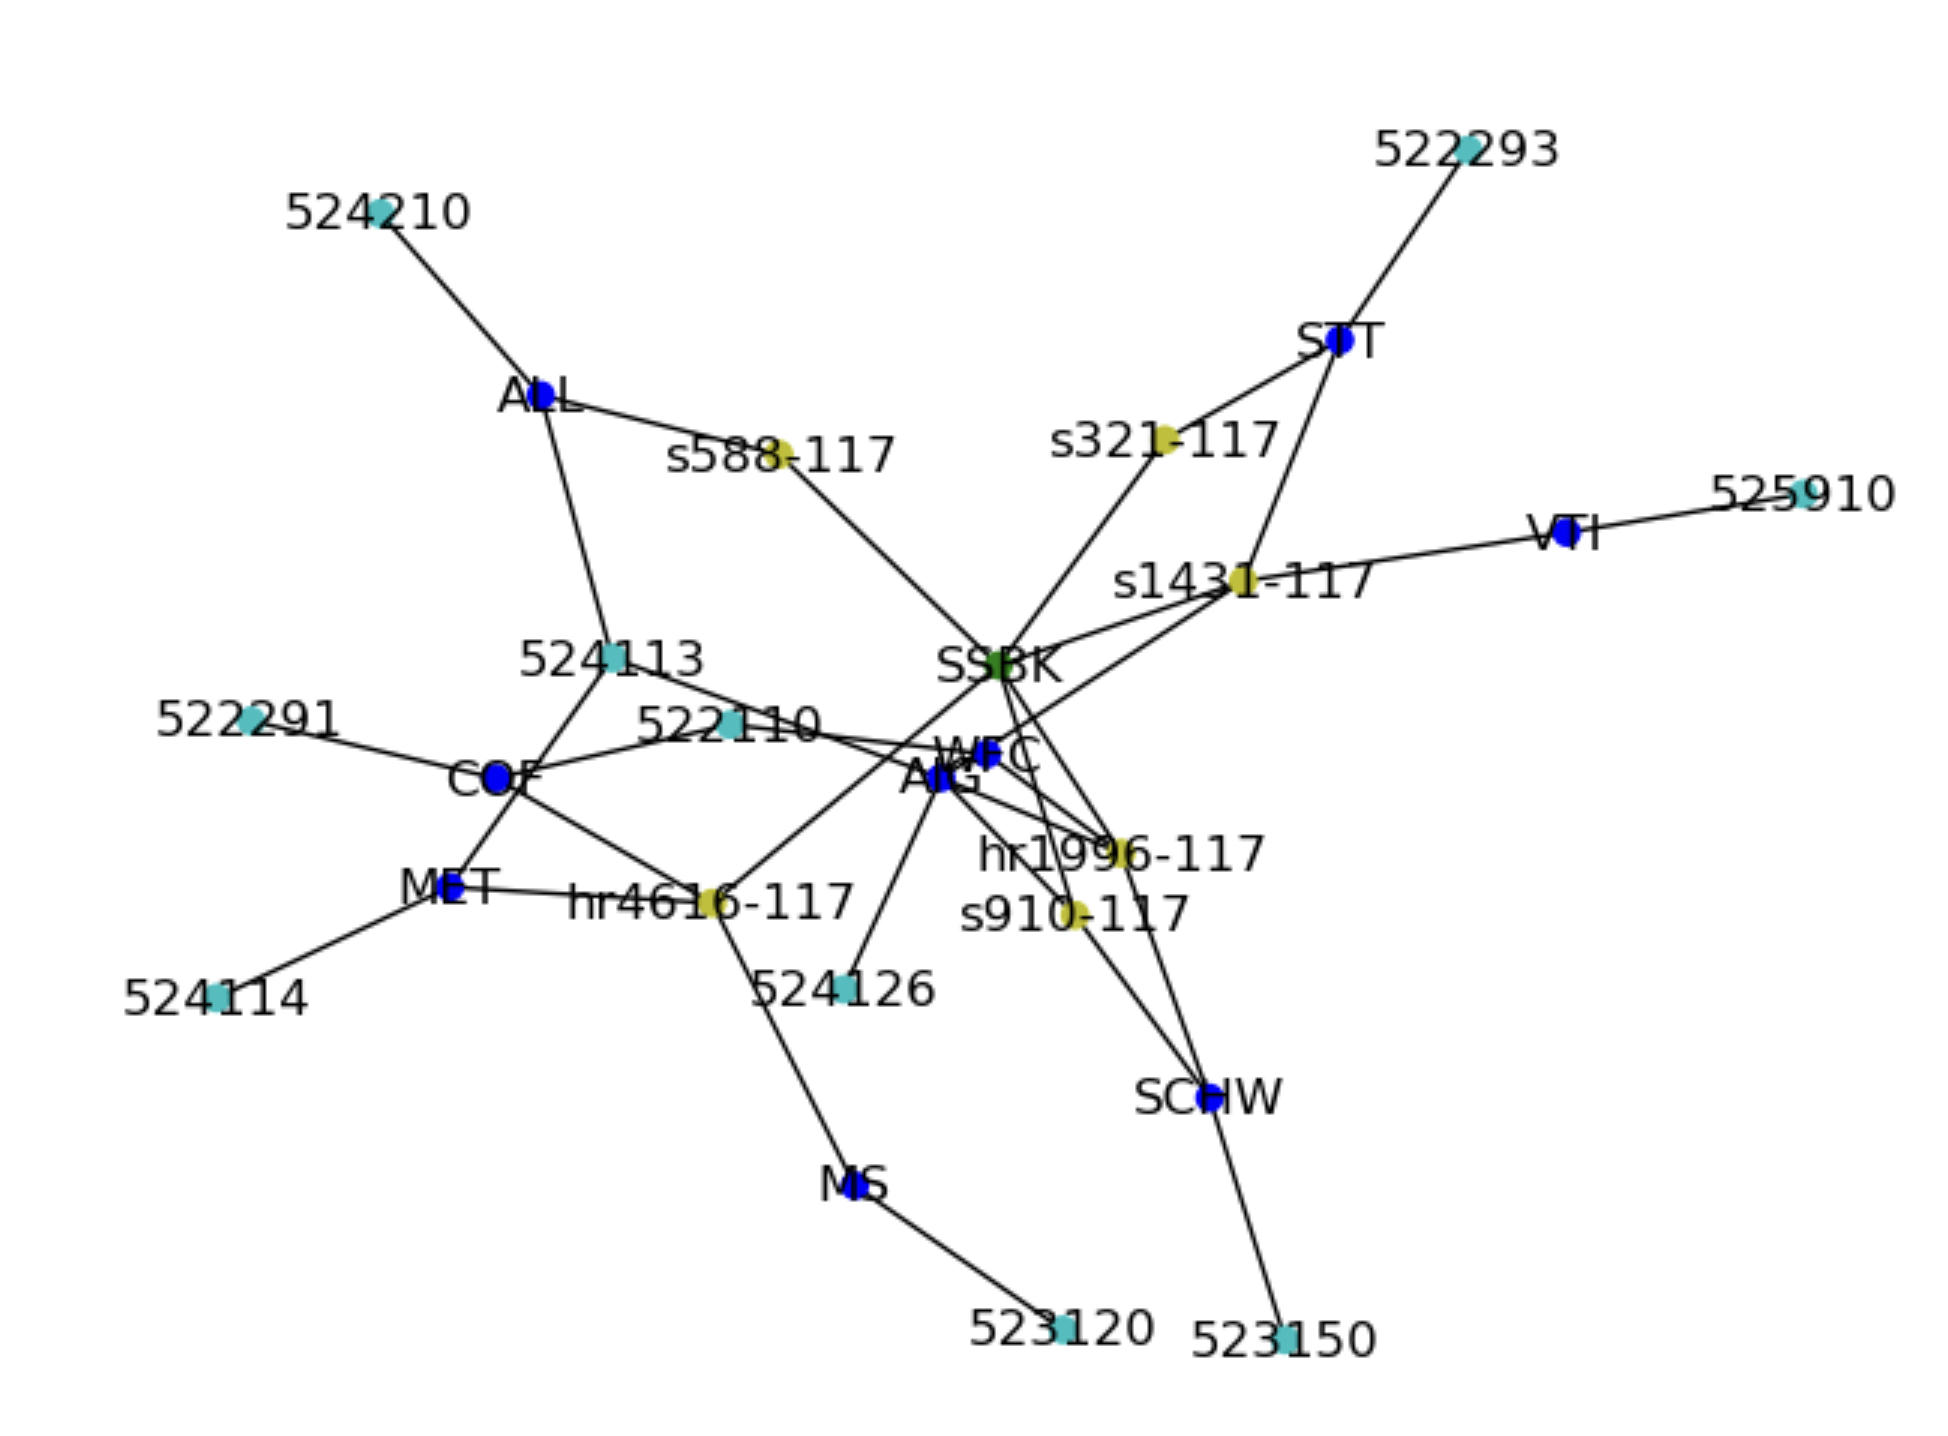
\includegraphics[width=1\textwidth]{imgs/SSBKs.png}
  \caption{\textbf{Subgraph capturing how the financial industry's interests were funneled through the Senate Banking Committee during the 117th Congress} the Senate Banking Committee (SSBK) serves as a channel for different financial companies to project their lobbying interests over bills. NAICS codes starting from 52 generally relate to the financial industry in Figure \ref{fig:ssbk}. For instance, Wells Fargo (WFC) and AIG are lobbying for H.R.1996 - SAFE Banking Act of 2021, which prohibits a federal banking regulator from penalizing a depository institution for providing banking services to a legitimate cannabis-related business. Capital One Inc. (COF) and MetLife Inc. (MET) are lobbying for H.R.4616, which allows for the transition of certain financial contracts away from the London Interbank Offered Rate (LIBOR). These bills are all funneled through the Senate Banking Committee, thus a committee member of SSBK is more likely to be equipped with in-depth knowledge of the financial industry.
  }
  \label{fig:ssbk}
\end{figure}


\subsection{Data Merging and Entity Disambiguation}

One of the key challenges in this study is the effective disambiguation of entities, as the data is collected from multiple sources, including LobbyView, Senate/House Financial Disclosures, and naics.com. In this graph-structured dataset, entities such as Congresspersons and firms may appear under different names or expressions. For example, "Ron Wyden" may also be referred to as "Ron L. Wyden," and "Apple" may appear as "Apple, Inc." To accurately analyze the relationships between these entities, it is essential to establish a unique identifier for each entity, regardless of the variations in their names.

Theoretically, matching entities based on text similarity between two datasets with $n$ and $m$ rows has a computational complexity of 
$O(n m)$. 
However, as the datasets grow larger, this complexity becomes prohibitively expensive. For instance, matching 70,000 firm names from LobbyView to 4,000 firm names appearing in the ticker table would require 280,000,000 text similarity computations. To address this challenge, I developed a novel approach that leverages URLs as unique identifiers for entities.

The approach involves acquiring the corresponding URL for each entity through Google searches, such as \url{https://en.wikipedia.org/wiki/Ron_Wyden} for Ron Wyden and \url{https://www.apple.com/} for Apple, Inc. A key advantage of using URLs as unique identifiers is that they facilitate effective entity disambiguation. For example, if two different expressions, "Ron Wyden" and "Ron L. Wyden," are both assigned the same URL \url{https://en.wikipedia.org/wiki/Ron_Wyden}, we can confidently recognize that these two expressions refer to the same entity. This approach allows us to accurately consolidate information about entities that may be represented in various ways across different data sources. Additionally, this method reduces the computational complexity to 
$O(n+m)$, as only one query is required for each row of data. To further scale up this process, I parallelized the URL acquisition process by batching queries and distributing them across multiple servers available through commercial cloud services like AWS.


In summary, this innovative approach to entity disambiguation through URL acquisition and parallelization enables efficient data merging from diverse sources, ensuring the accuracy and scalability of the analysis.

\subsection{Effective Parsing Technique for Financial Disclosures}

Financial Disclosures from the House are provided as encrypted PDF files. While text can be extracted from these files, the encryption results in irregular patterns, particularly in the tables that contain information about Congresspersons' stock buying and selling activities. These irregular patterns make it challenging to parse the data using manually coded patterns, as the deviations are difficult to anticipate and account for. To address this challenge, I utilized OpenAI's APIs, specifically the GPT-3.5 Turbo language model, to parse the PDFs into a CSV format that includes information such as when and who bought or sold which ticker, and how much.

The process involves querying the Large Language Model (LLM) with the extracted text from the PDFs and instructing the model to convert the irregularly formatted tables into structured CSV data. The CSV format includes columns such as the date of the transaction, the name of the Congressperson, the ticker symbol of the stock, the type of transaction (buy or sell), and the amount of the transaction.

By leveraging the capabilities of the GPT-3.5 Turbo language model, I was able to effectively parse information contained in PDF files that would normally require manual human labor. This approach significantly streamlines the data extraction process and ensures the accuracy and consistency of the parsed data.

\section{Estimating Excess Returns at the Congressperson-Ticker Level} \label{ex-r}

The broader literature on insider trading has long explored the information advantages that certain individuals, such as corporate insiders or well-connected investors, may possess when trading in the stock market. For example, Jeng et al. (2003) estimated returns to insider trading from a performance-evaluation perspective, while Ivković and Weisbenner (2005) studied the information content of the geography of individual investors' common stock investments. These studies highlight the importance of understanding the impact of information asymmetry and potential insider trading in financial markets.

Despite the extensive research on insider trading in general, the application of this approach to congressional stock trading has been limited. In the context of congressional stock trading, previous studies, such as those conducted by Ziobrowski (2004, 2011) and Egger \& Hainmueller (2013), have predominantly used calendar-time based portfolio approaches (
  Hoechle, D., M. Schmid, and H. Zimmermann. 2009) to estimate excess returns. This involves creating synthetic buy and sell portfolios that mimic congresspersons' stock purchases and sales but sell or buy such stocks after a year. However, this approach masks the importance of transaction timing, which is a crucial aspect of insider trading (Tahoun, 2014, Schweizer, 2011), as it fails to account for short-term fluctuations in stock prices that may be driven by the congresspersons' access to privileged information. This presents a severe limitation in understanding the true extent of potential insider trading among U.S. members of Congress.

Moreover, averaging excess returns across congresspersons may not capture the full extent of insider trading within the Beltway, 
the inner circle of Washington D.C. politics. Schweizer (2011) provided anecdotal evidence of politicians and their friends profiting from insider stock tips, 
while Lenz \& Lim (2010) studied corruption and wealth accumulation in Congress, and Jerke (2010) and Bainbridge (2010) 
examined the use of political intelligence for profit and insider trading inside the Beltway, respectively. 
These case studies suggest that certain congresspersons might engage in insider trading with specific firms or industries,
 which would be overlooked in an aggregate analysis.

In this section, we aim to address these limitations by estimating the excess returns at the congressperson-ticker level, with a focus on the life cycle of each buy/sell chain of specific tickers consecutively transacted by a congressperson. This approach offers a more granular analysis of potential insider trading among U.S. members of Congress, allowing us to better evaluate whether widespread insider trading exists at the congressperson-ticker level. By doing so, we build upon both the general insider trading literature and the existing research on congressional stock trading, contributing to a more comprehensive understanding of the potential information advantages leveraged by politicians in the stock market and the importance of transaction timing.


\subsection{Uncanny Timing of Investments of Congressmen} \label{prelim}

Firstly, I gained insights into the mechanisms behind their trading decisions by reviewing news articles. For example, there were several media reports\footnote{\url{https://nypost.com/2021/05/20/us-sen-ron-wyden-boosts-chipmakers-while-his-wife-buys-their-shares/}} in May 2021 regarding Ron Wyden's semiconductor stocks trading.
I searched for Senator Ron Wyden's stock transactions that occurred prior to May 2021, but within a year, with a NAICS code beginning with 334, which indicates computer and electronic product manufacturing.
I found that three different tickers (AMAT, AVGO, KLAC) of the transactions that met this condition have a commonality in that they all started on the same date, April 6th, 2020, and ended on either April 6th or April 16th, 2021. Furthermore, all of them follow a similar pattern of multiple purchases followed by sales after certain critical points, such as $Purchase-Purchase- \hdots - Purchase \text{ } |  \text { } Sales - Sales - \hdots - Sales$ as shown in Fig \ref{fig:trans}.

\begin{figure}[h]
  \centering
  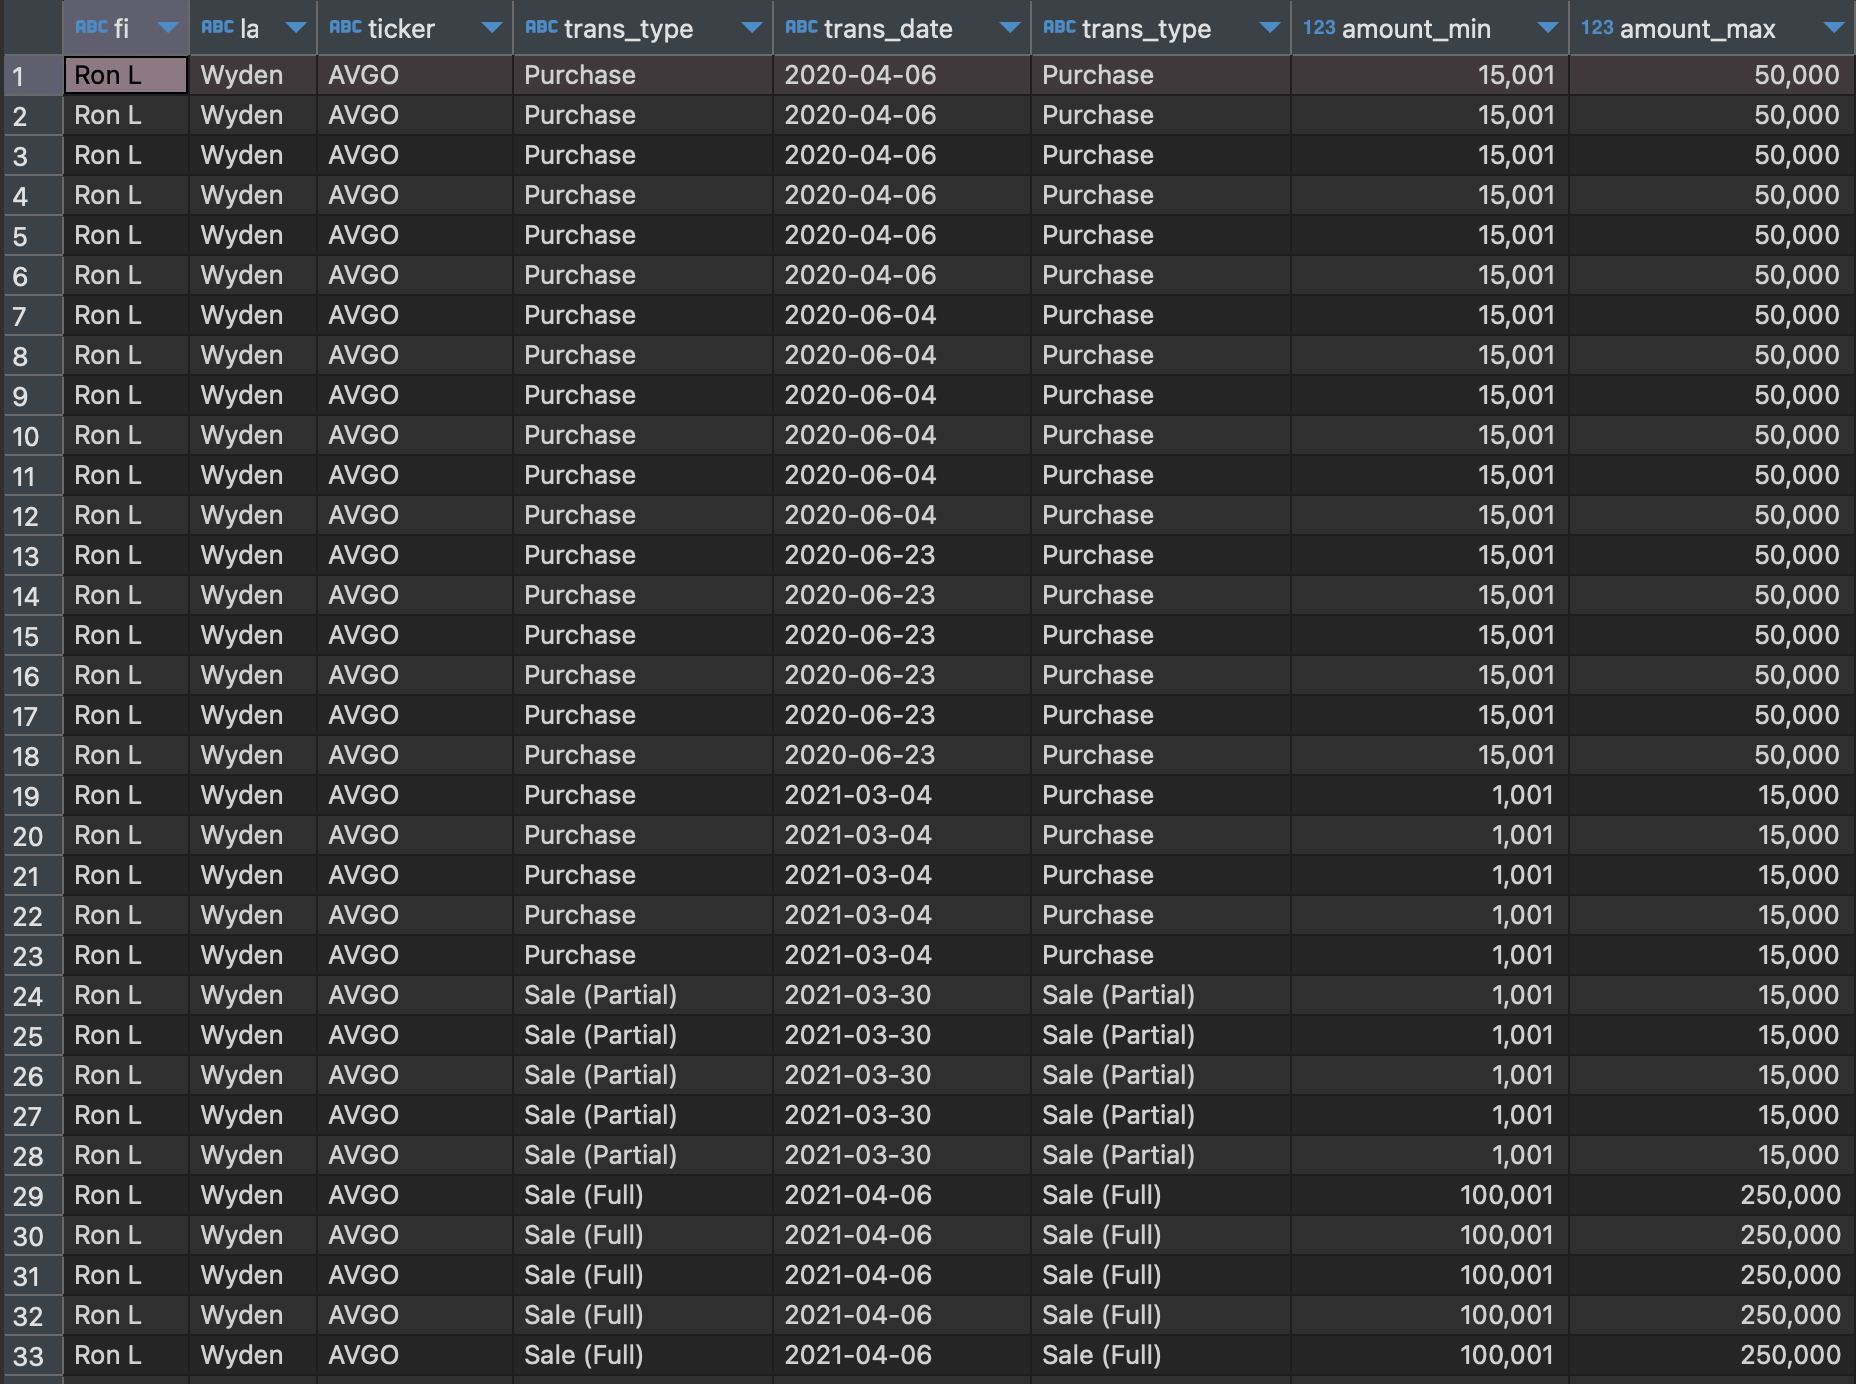
\includegraphics[width=1\textwidth]{imgs/trans.png}
  \caption{Senator Ron Wyden's stock transactions for Broadcom Inc. (ticker AVGO) exhibited a pattern of multiple purchases followed by sales after certain critical points, spanning from April 6th, 2020 to April 6th, 2021.}
  \label{fig:trans}
\end{figure}

On April 1st, 2021, President Biden announced a plan to invest \$50 billion to boost the U.S. chip industry\footnote{https://www.wsj.com/articles/biden-urges-50-billion-to-boost-chip-manufacturing-in-u-s-11617211570}. After this announcement, Senator Ron Wyden sold all of his semiconductor stocks. This suggests that members of Congress may have access to legislative information that can impact certain industries and enable them to design their own portfolio based on this information, potentially resulting in profitable stock trades.

Based on this observation, I developed an algorithm to calculate the excess returns for each (Senator, Ticker) pair. Unlike previous literature \citep{zi11, zi24,eg13} that computes excess returns at the year-chamber level, such as the excess return of the Senate or House over a specific year, I hypothesized that insider trading occurs in a time-specific manner. Therefore, it should be estimated accordingly, rather than a year-based approach. As a result, I selected all transaction chains that start with multiple purchases followed by sales within six months of the transition from purchase to sale.

There is a methodological challenge with using the Senate Finance Disclosure data, as it only provides the minimum and maximum range of amounts spent on purchasing or selling each ticker on a specific day (See Figure \ref{fig:trans}). To estimate the distribution of excess returns for each particular Purchase-Sale chain at the (Senate, Ticker) level, I randomly sampled the amount from a uniform distribution with support equal to the min/max range of the amount in the data. To obtain a more conservative estimate of the excess return, I penalized the monetization of a unit stock by the average Federal Reserve Rate during the holding period, even though the savings account rate is typically lower.

I am presenting the excess return distributions for Senator Ron Wyden's transactions involving two companies: Applied Materials Inc. (AMAT), which provides manufacturing equipment, services, and software to the semiconductor industry, and Marriott International Inc. (MAR), a global hotel brand. These distributions were computed using the random sampling method explained earlier. The X-axis of Figure 4 represents the percentage of return for a unit investment, with a value of 120 indicating a gain of \$1.20 for every \$1 invested.
\begin{figure}[htbp]
  \centering
  \begin{subfigure}[t]{0.45\textwidth}
  \centering
  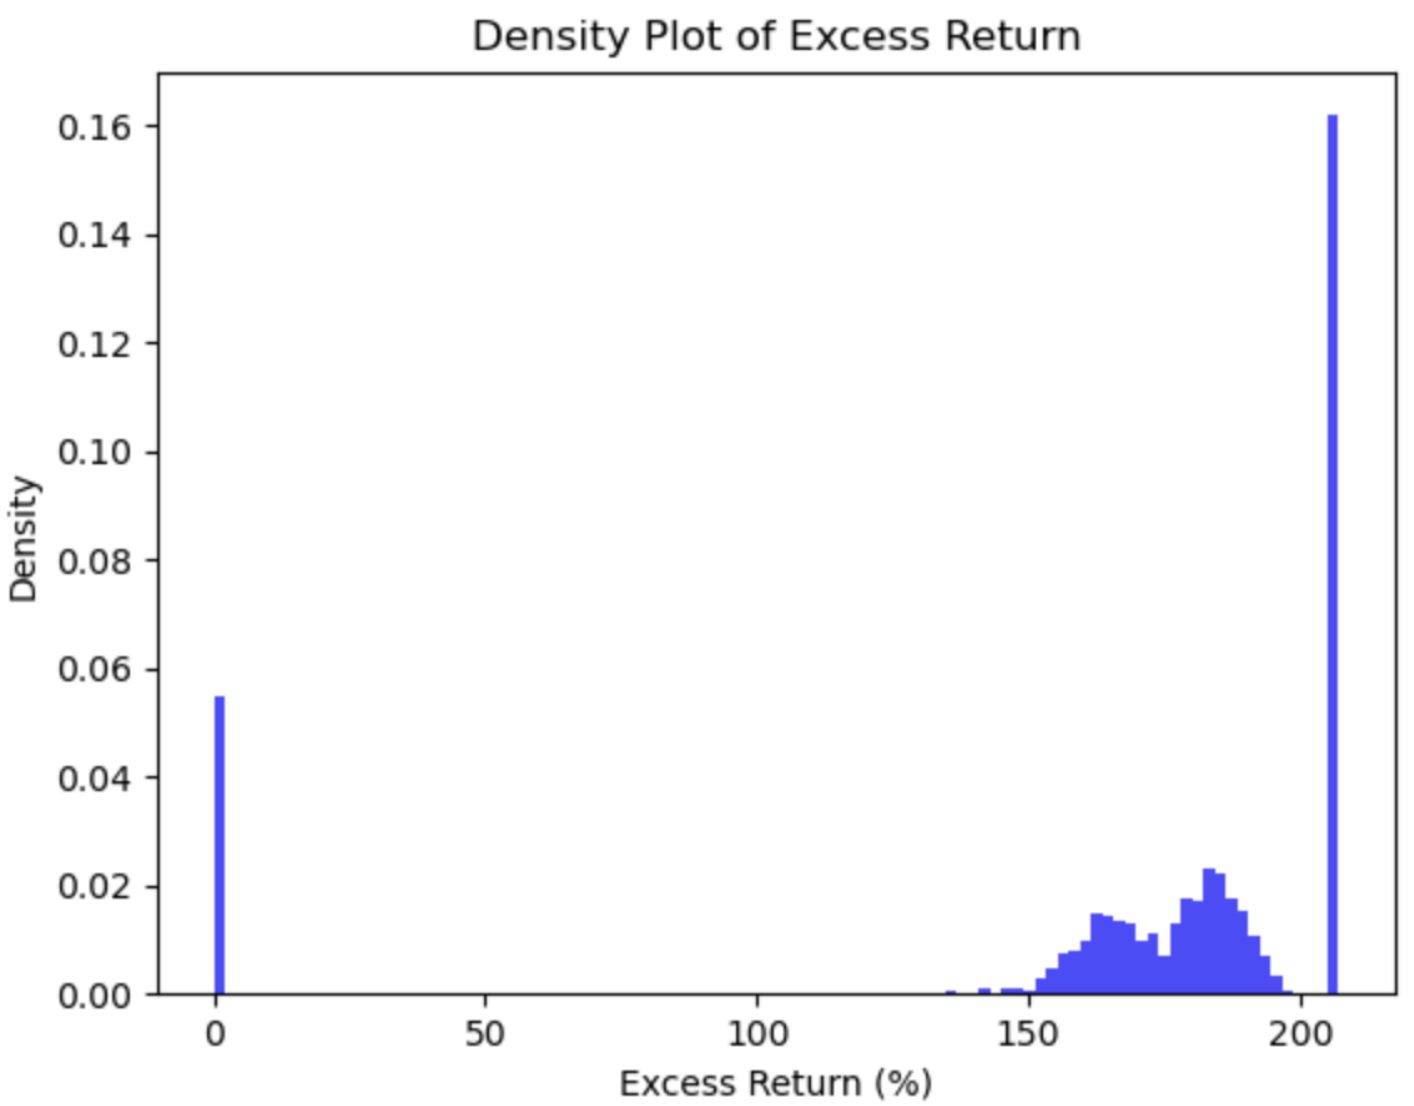
\includegraphics[width=\textwidth]{imgs/RWAMAT.png}
  \caption{Ron Wyden's excess returns from transactions involving Applied Materials Inc. (AMAT) from April 2020 to April 2021.}
  \label{fig:er_klac}
  \end{subfigure}
  \hfill
  \begin{subfigure}[t]{0.45\textwidth}
  \centering
  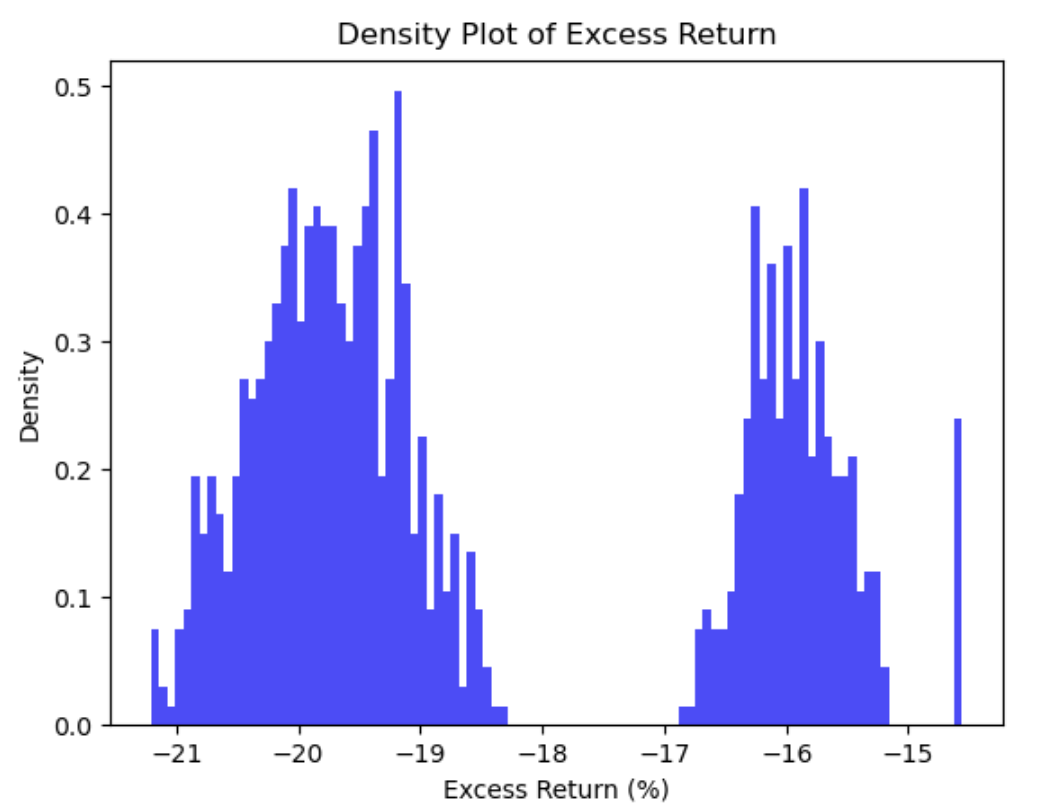
\includegraphics[width=\textwidth]{imgs/RWMAR.png}
  \caption{Ron Wyden's excess returns from transactions involving Marriott International Inc. (MAR) from May to August 2020.}
  \label{fig:er_mar}
  \end{subfigure}
  \caption{Excess return distributions of Senator Ron Wyden's transactions for AMAT and MAR
  }
  \label{fig:er}
\end{figure}

As shown in Figure 5, it appears that Senator Ron Wyden may have access to legislative information regarding bills that could impact both the semiconductor and hospitality industries. During the 117th Congress, which coincides with Senator Ron Wyden's transaction involving AMAT, the company lobbied for two bills: S.2107 FABS Act and S.749 American Innovation and Jobs Act. Both bills include provisions that provide subsidies to the semiconductor industry. Additionally, during the 117th Congress, which overlaps with Senator Ron Wyden's transaction involving MAR, the company lobbied for two bills: S.477 Hospitality and Commerce Job Recovery Act of 2021, which extends tax credits to assist the hospitality and restaurant industry, and S.1519, which grants awards to hotel owners. It is worth noting that this legislative information likely flowed from the firms' lobbying efforts directed towards the Senate Finance Committee, which oversees the bills listed.
\begin{figure}[htbp]
  \centering
  \begin{subfigure}[t]{0.45\textwidth}
  \centering
  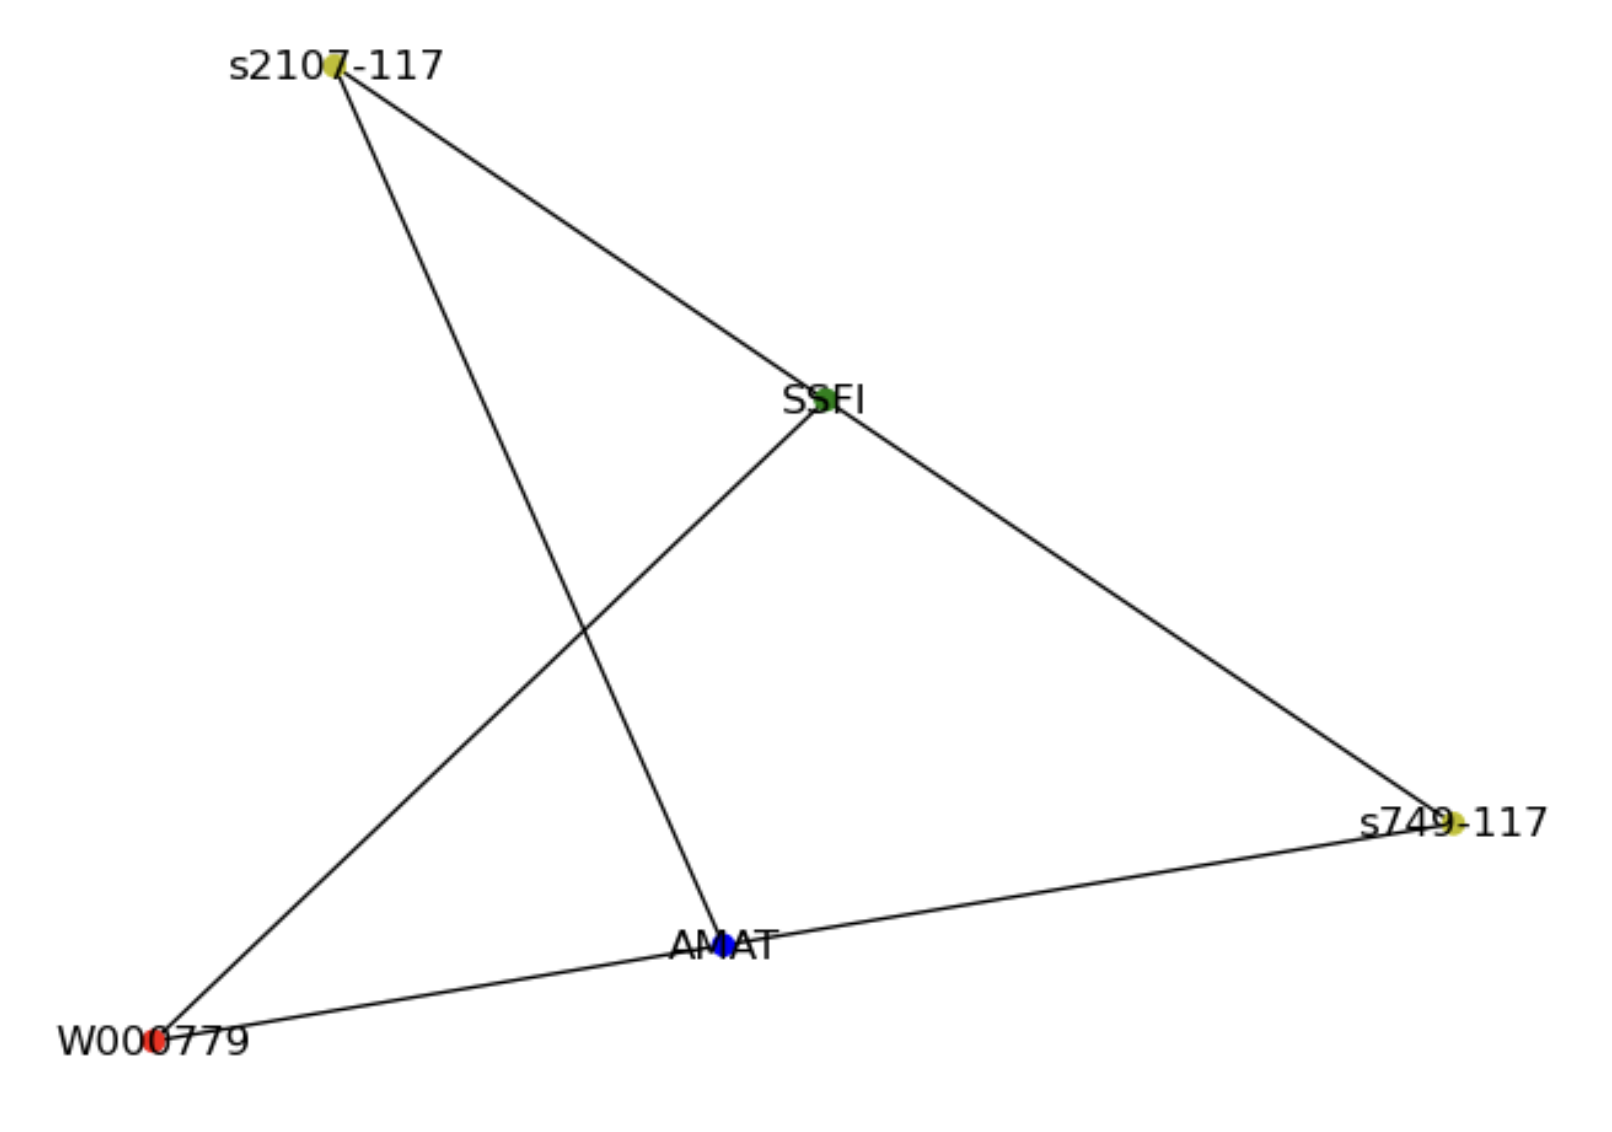
\includegraphics[width=\textwidth]{imgs/AMATDAG.png}
  \caption{Subgraph extracted from the congressional network that is in close proximity to Senator Ron Wyden's purchase or sale transaction involving AMAT.}
  \label{fig:er_klac}
  \end{subfigure}
  \hfill
  \begin{subfigure}[t]{0.45\textwidth}
  \centering
  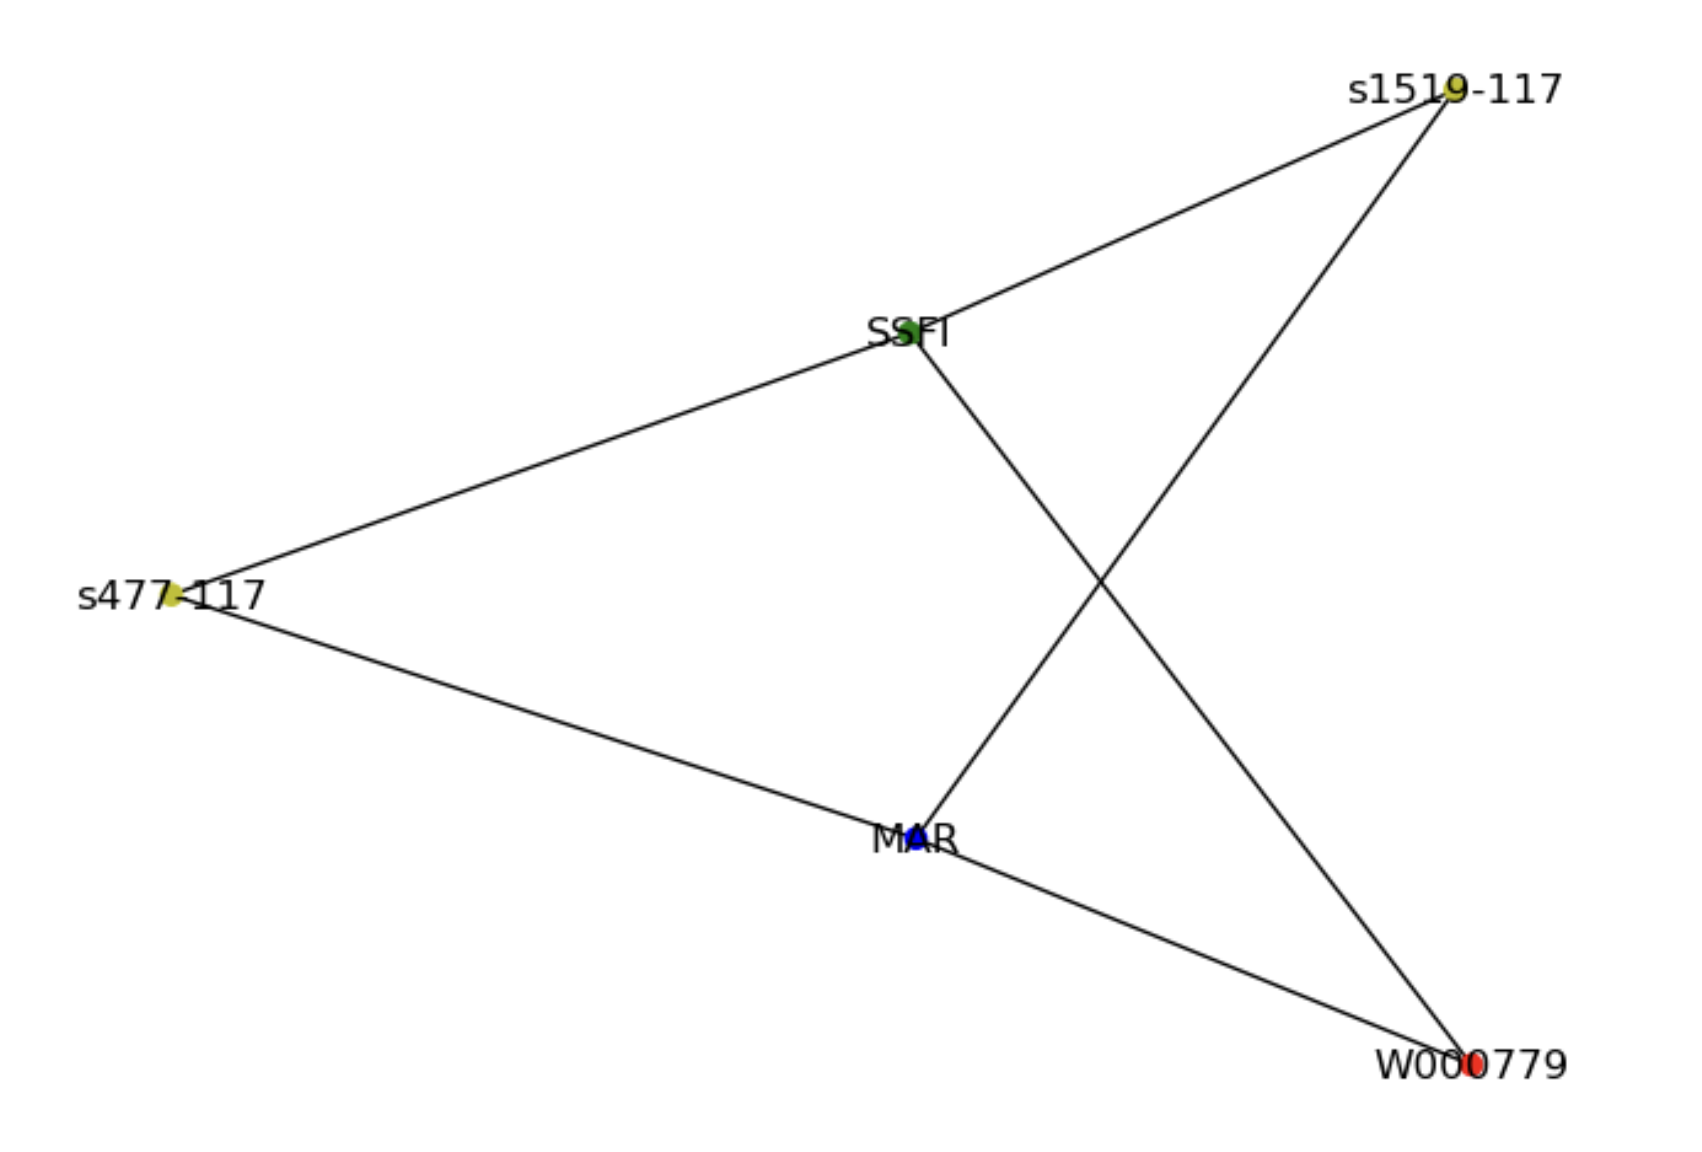
\includegraphics[width=\textwidth]{imgs/RWMAR2.png}
  \caption{Subgraph extracted from the congressional network that is in close proximity to Senator Ron Wyden's purchase or sale transaction involving MAR.}
  \label{fig:er_mar}
  \end{subfigure}
  \caption{Potential Access to Legislative Information by Senator Ron Wyden Regarding Bills Impacting Semiconductor and Hospitality Industries during the 117th Congress
  }
  \label{fig:er2}
\end{figure}


Based on both Figure \ref{fig:er} and Figure \ref{fig:er2}, we can conclude that although Senator may have access to legislative information about certain industries, it is not always possible to profit from it due to external factors that the legislative information from congressional activity cannot explain. This example provides suggestive evidence as to why a simple excess return approach cannot provide a persuasive argument that proves or disproves the existence of insider trading.  

Finally, I provide a distribution of the mean estimated excess return for each (Senator, Ticker) pair in Figure \ref{fig:erfin}. The plot shows that only a few transactions are acquiring abnormal positive profits over 50\%, and almost half of them record negative returns. This statistic is consistent with the findings reported by \cite{eg13}, which suggests that there is little evidence of systematic abnormal returns for members of Congress. However, thanks to the current approach that delves more into the Senator and Ticker level, we can conclude that it is hard to deny that a few transactions are acquiring abnormally high returns connected to the relevant legislative information that is accessible during congressional activity.

\begin{figure}[h]
  \centering
  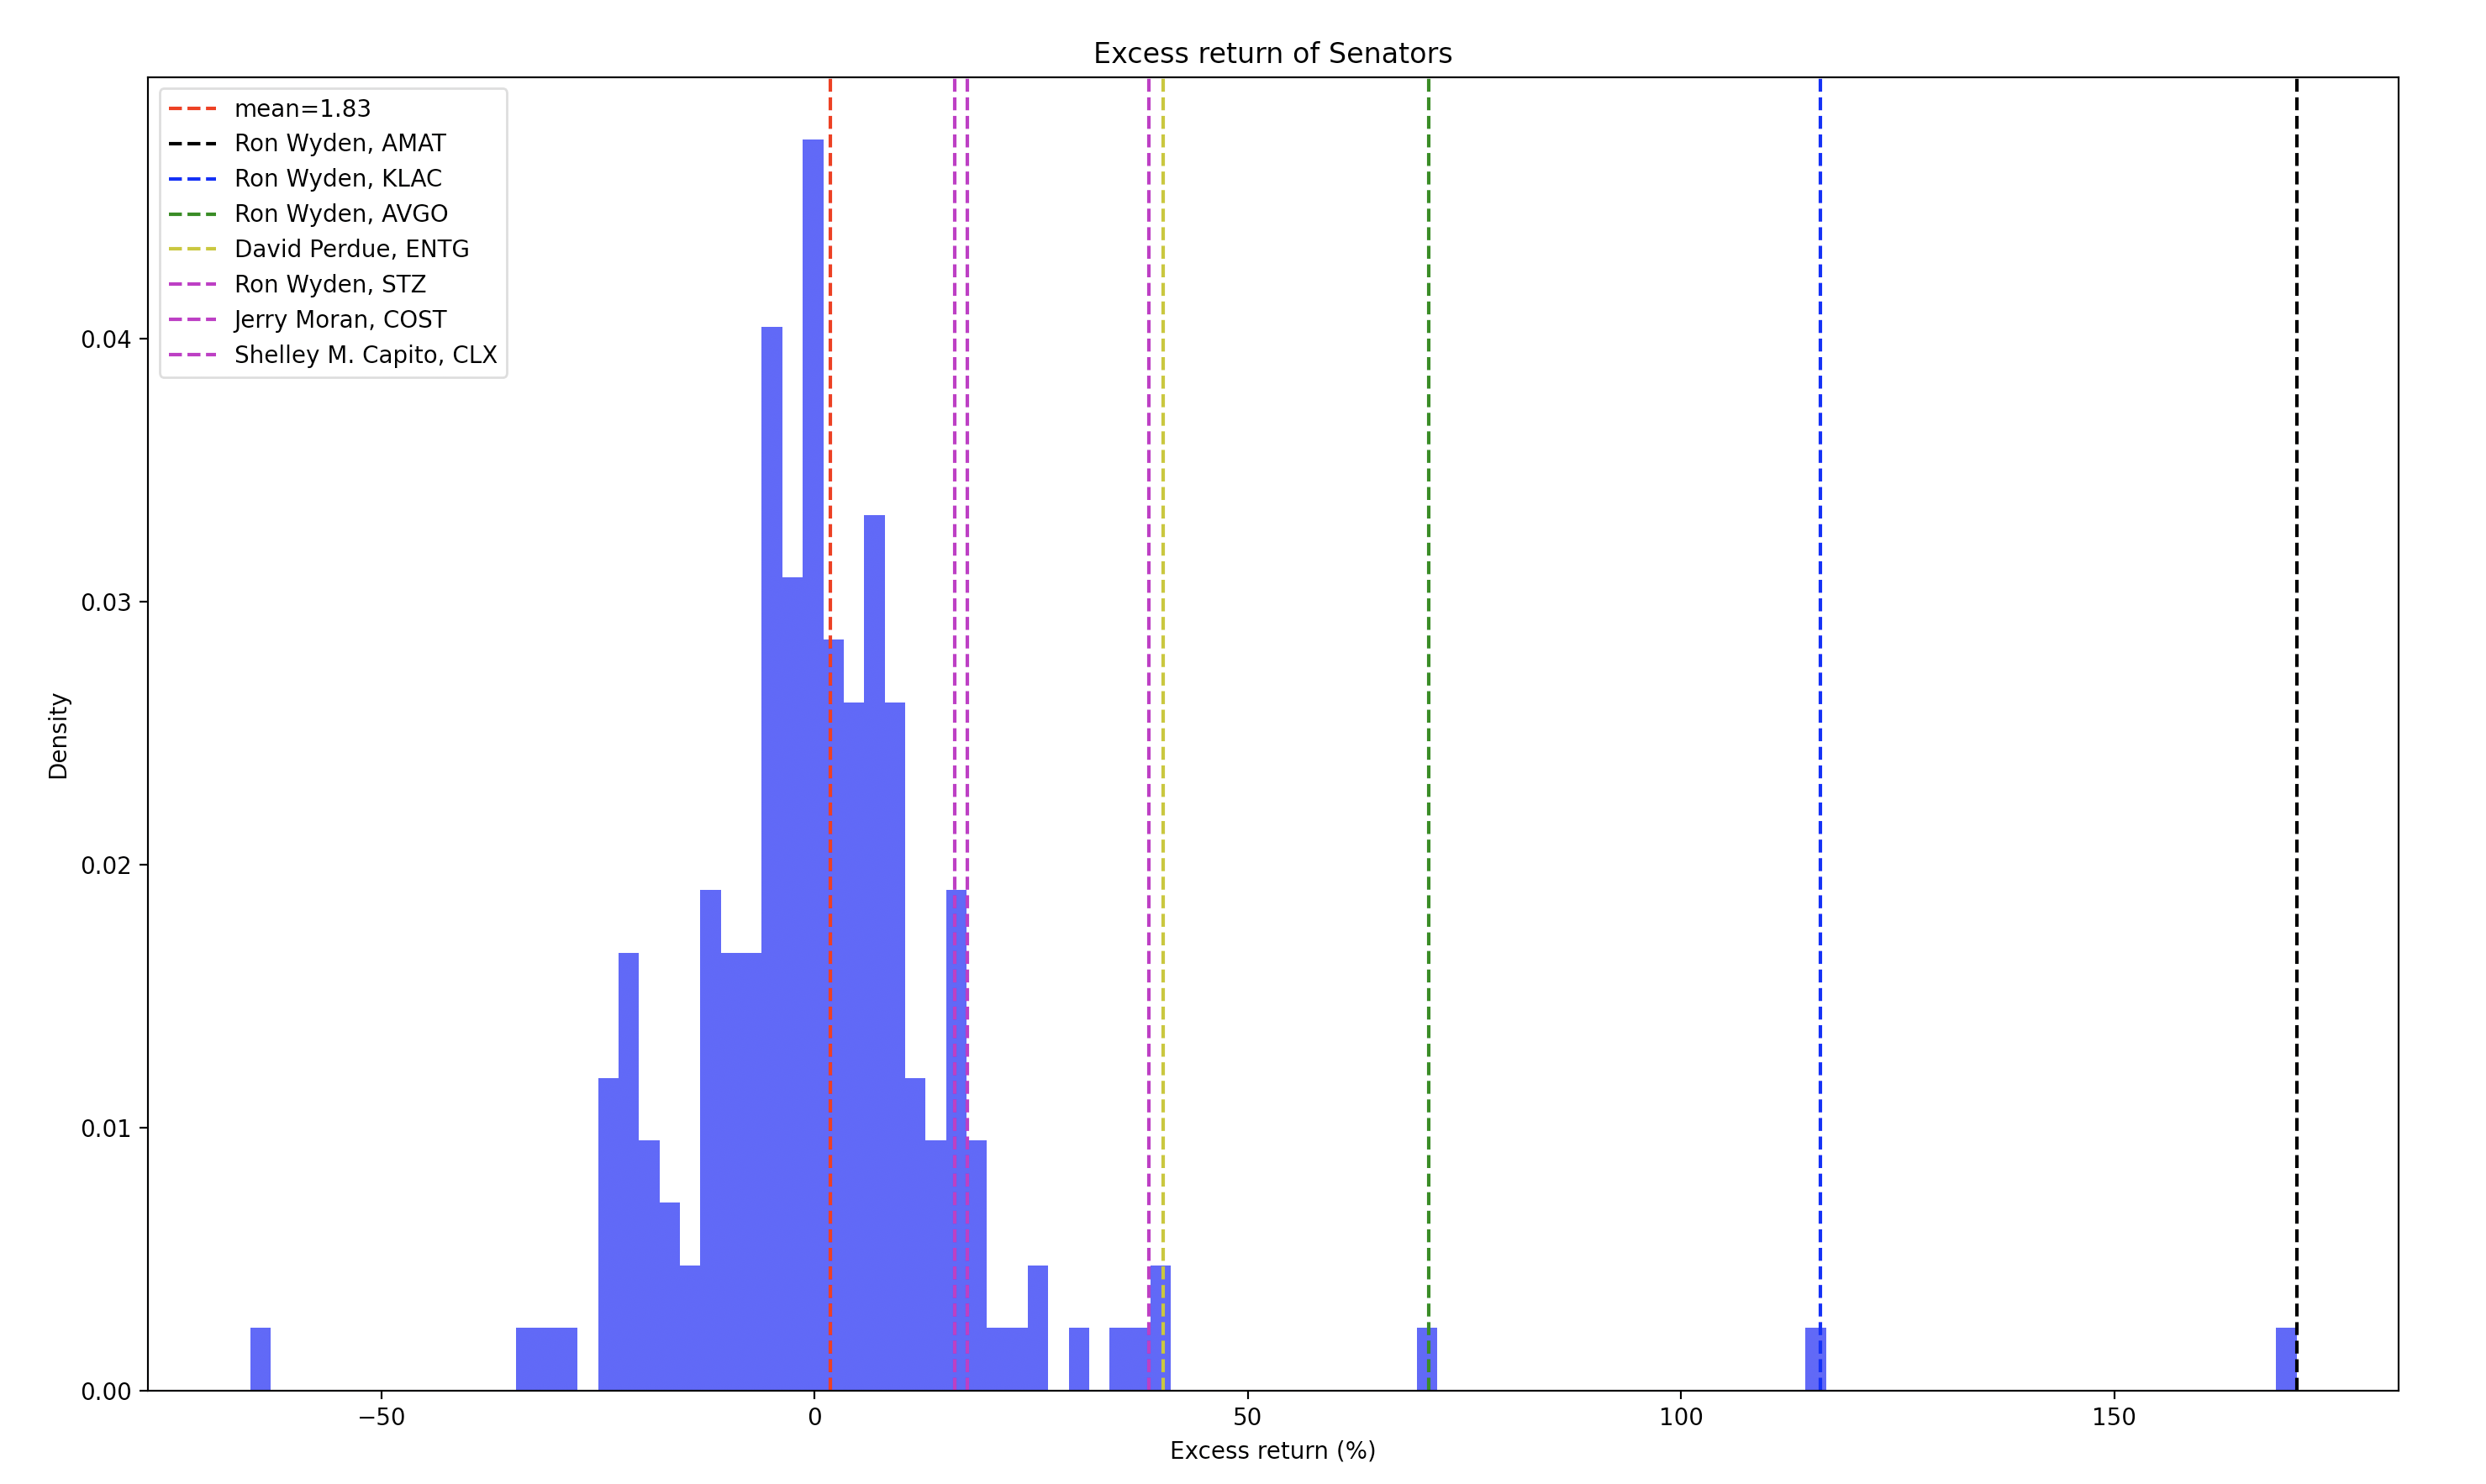
\includegraphics[width=1\textwidth]{imgs/ERFin.png}
  \caption{Distribution of congressmen's excess returns at the Senate-ticker level.}
  \label{fig:erfin}
\end{figure}

% \subsection{Committees: A Channel for Legislators to Acquire Industry-Specific Information}\label{comm}
% Based on multiple anecdotes and observations, I hypothesize that legislators acquire industry-specific information from their committee assignments that they may use for personal investments. For example, Senator Ron Wyden's semiconductor stock transactions involving multiple tickers in the same industry, such as AMAT, AVGO, and KLAC, can be explained by this hypothesis. These companies lobbied for bills relevant to the semiconductor industry, and the industry-level preferences and possible impacts of legislation on the semiconductor industry were aggregated in the Senate Finance Committee, which oversees such bills. As a member of the Senate Finance Committee, Ron Wyden acquired a more detailed understanding of how vital these bills were to the industry, and may have timed his transactions accordingly.
I also provide an additional illustration that shows how the preferences of the semiconductor industry were focused on the Senate Finance Committee during the 117th Congress in Figure \ref{fig:semi}. The NAICS code 334413 indicates Semiconductor and Related Device Manufacturing, which involves companies such as Qualcomm (QCOM), Intel (INTC), IBM (IBM) and Advanced Micro Devices (AMD), lobbying for bills such as the CHIPS Act and FABS Act that are closely related to the subsidization of semiconductor manufacturing facilities. Relevant companies such as Apple Inc. and IBM, with NAICS codes of 334220 Wireless Communications Equipment Manufacturing and 334118 Computer Equipment Manufacturing, respectively, are direct customers of these semiconductor chips for manufacturing smartphone and computer hardware. The bills in which these companies have an interest are assigned to the Senate Finance Committee as well.



As another example, I provide how the Senate Banking Committee (SSBK) serves as a channel for different financial companies to project their lobbying interests over bills. NAICS codes starting from 52 generally relate to the financial industry in Figure \ref{fig:ssbk}. For instance, Wells Fargo (WFC) and AIG are lobbying for H.R.1996 - SAFE Banking Act of 2021, which prohibits a federal banking regulator from penalizing a depository institution for providing banking services to a legitimate cannabis-related business. Capital One Inc. (COF) and MetLife Inc. (MET) are lobbying for H.R.4616, which allows for the transition of certain financial contracts away from the London Interbank Offered Rate (LIBOR). These bills are all funneled through the Senate Banking Committee, thus a committee member of SSBK is more likely to be equipped with in-depth knowledge of the financial industry.

% \subsection{Causal Quantity of Interest: Effect of Committee Membership on Trading Behavior}

% In Section \ref{comm}, illustrative examples were provided to suggest that committee assignments can influence a congressman's financial behavior by utilizing industry-level specialized information funneled through the committee. Building on this insight, I propose a Directed Acyclic Graph (DAG) in Figure \ref{fig:dag} that captures the hypothesized causal relationships between committee assignments, congressional knowledge, and financial behavior. Specifically, I expect that Congressional Knowledge before joining a committee will act as a confounder, influencing both the committee assignment and financial behavior. After joining the committee, Congressional Knowledge will mediate the effect of the committee assignment on financial behavior. At the outcome level, I expect that the industry distribution of a senator's portfolio after joining the committee will become more similar to that of the committee. The industry distribution of the committee will be evaluated by examining the firms' industry distribution lobbying for bills assigned to that committee.

% \begin{figure}[h]
%   \centering
%   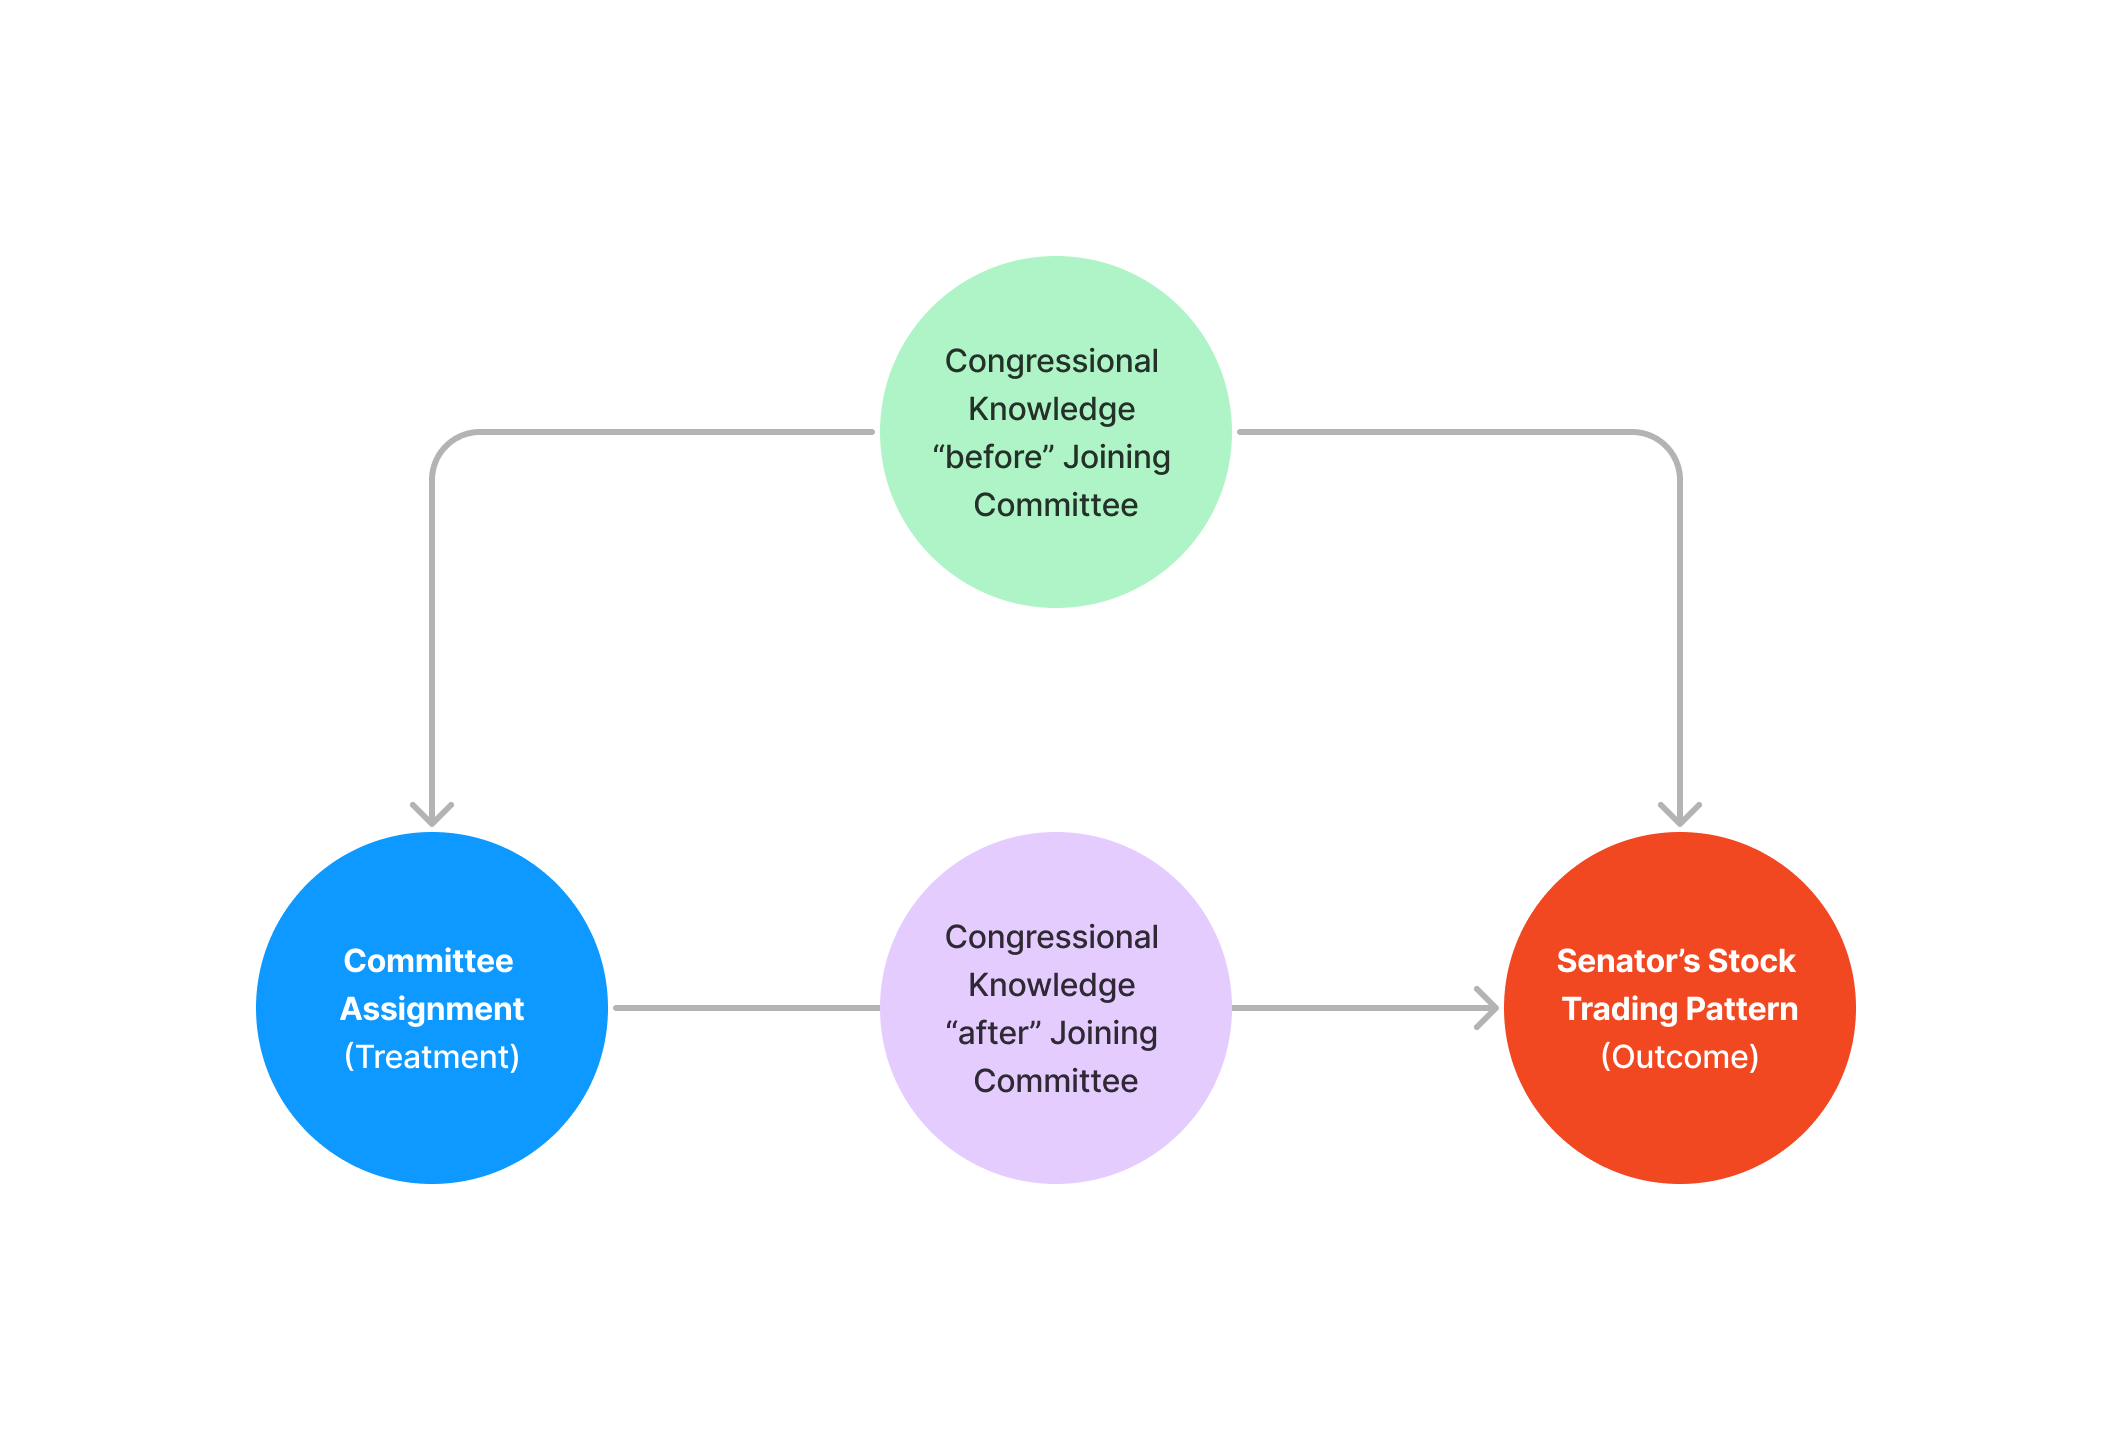
\includegraphics[width=1\textwidth]{imgs/causaldag.png}
%   \caption{Causal diagram that demonstrates how committee assignments affect the congressmen's transaction behavior}
%   \label{fig:dag}
% \end{figure}

% To justify the measurement of the outcome variable as a similarity between the industry-level distribution of a senator's stock trading portfolio and that of the committee, I analyzed the stock trading portfolio and its NAICS code distribution for Senator Ron Wyden, as well as those of the Senate Finance Committee (SSFI) and Senate Banking Committee (SSBK) over the 117th Congress, as shown in Figure 8. I calculated the discrete probability distribution of the collection of 2-digit level NAICS codes for each entity, and used cross-entropy to measure the similarity between the Senator and each committee's NAICS code distribution. The results indicate that the cross-entropy between Senator Ron Wyden's NAICS code distribution and that of SSFI is 0.71, while the cross-entropy between Senator Ron Wyden's NAICS code distribution and that of SSBK is 3.31. 
% A smaller cross-entropy value signifies a more similar distribution, indicating that Senator Ron Wyden's NAICS code distribution is closer to that of SSFI than SSBK. This supports the hypothesis that committee assignments influence a senator's investment choices, as Ron Wyden is a member of SSFI but not a member of SSBK.

% \begin{figure}[ht]
%   \centering
%   \begin{subfigure}[b]{0.3\textwidth}
%     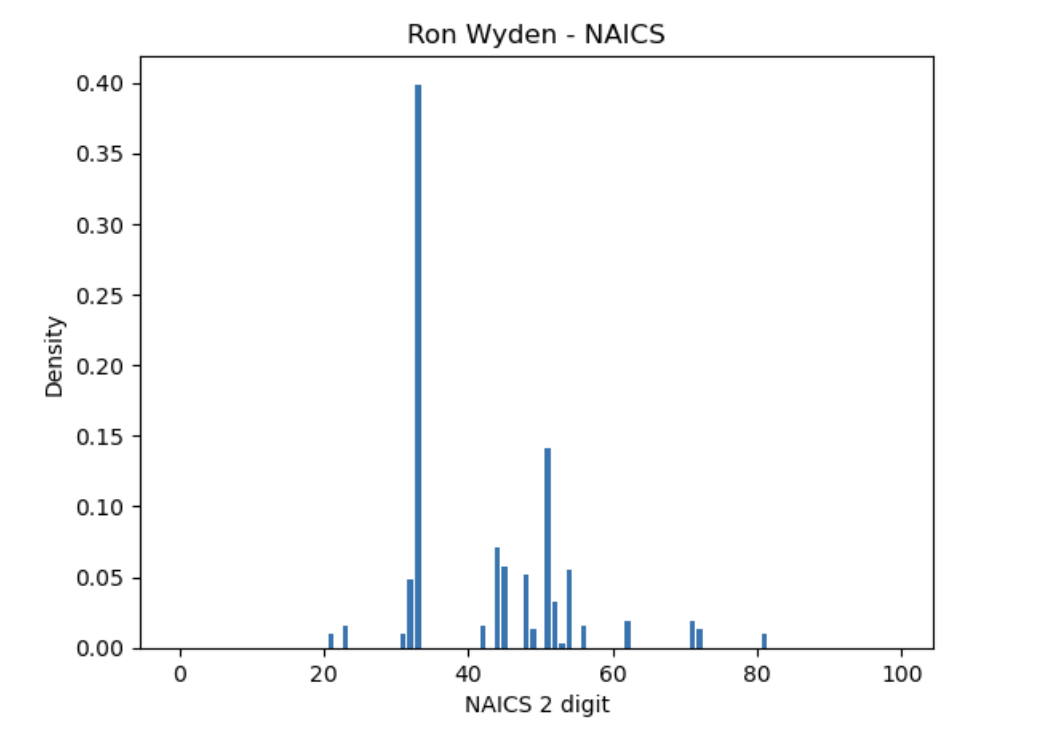
\includegraphics[width=\textwidth]{imgs/naics1.png}
%     \caption{NAICS code distribution of Senator Ron Wyden's stock portfolio over the 117th Congress.\\}
%     \label{fig:subfig1}
%   \end{subfigure}
%   \hfill
%   \begin{subfigure}[b]{0.3\textwidth}
%     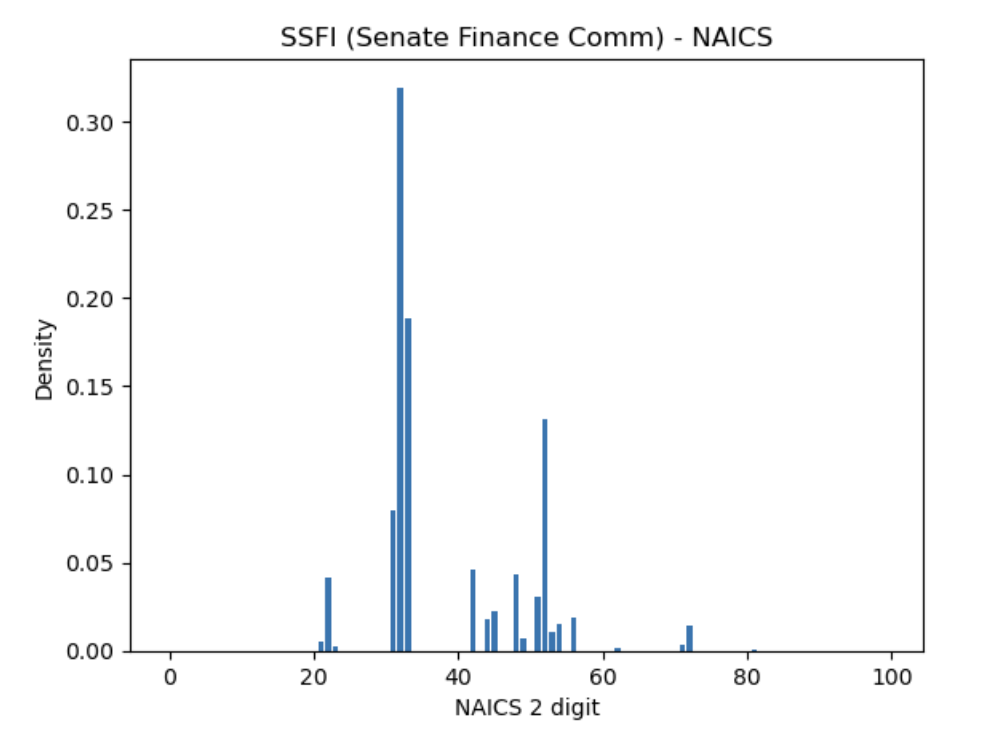
\includegraphics[width=\textwidth]{imgs/naics2.png}
%     \caption{NAICS code distribution of firms lobbying for bills assigned to Senate Finance Committee in the 117th Congress.}
%     \label{fig:subfig2}
%   \end{subfigure}
%   \hfill
%   \begin{subfigure}[b]{0.3\textwidth}
%     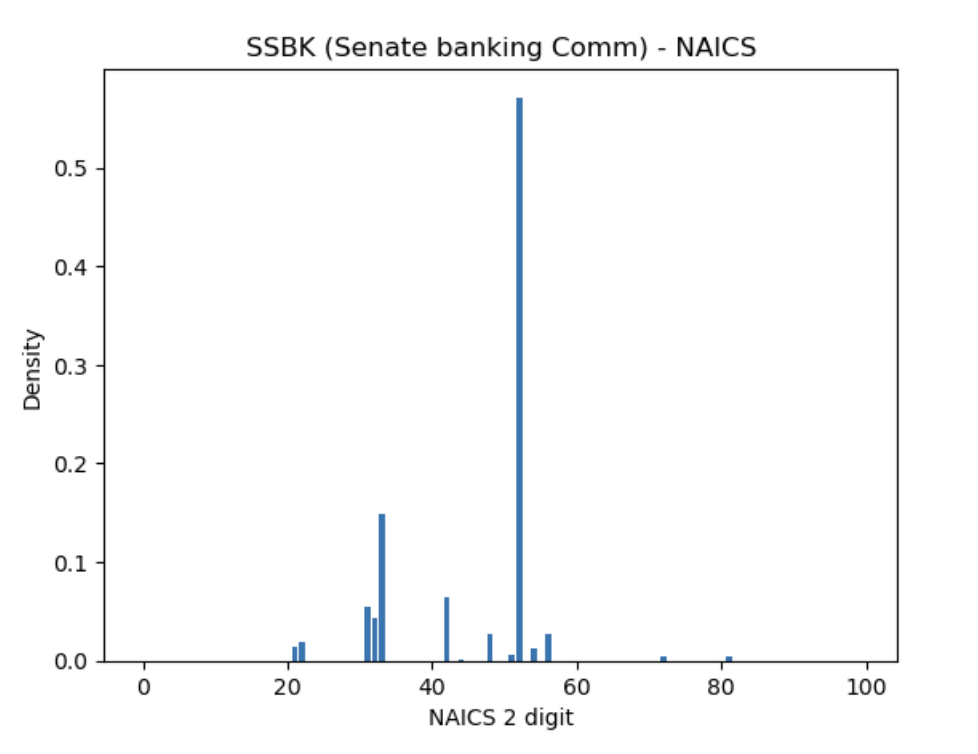
\includegraphics[width=\textwidth]{imgs/naics3.png}
%     \caption{NAICS code distribution of firms lobbying for bills assigned to Senate Banking Committee in the 117th Congress.}
%     \label{fig:subfig3}
%   \end{subfigure}
%   \caption{NAICS code distribution of Senator and Committees.}
%   \label{fig:mainfig}
% \end{figure}

% Therefore, I conclude that by estimating the causal effect of committee assignment on the cross-entropy between committees and senators, we can determine whether the information funneled through committee in congressional activity, after joining such committee, affects congressmen's trading behavior or not, provided that we properly control for the level of congressional knowledge before joining the committee.

% Then there exists a remaining question: how to measure congressional knowledge ``before'' joining a committee? Before proceeding, I assume that the congressional network $G$ described in Section \ref{data} is a comprehensive source of relevant information, meaning that it is sufficient to satisfy the backdoor-adjustment criterion for correctly estimating the causal effect of committee assignment on the outcome. However, although $G$ includes this sufficient information, we need to separate the congressional knowledge ``before'' and ``after'' joining the committee. Additionally, there is another challenge: $G$ is a discrete object that cannot be directly used in any model to estimate the quantity of interest in its raw format. To overcome these challenges, I suggest using Graph Neural Network (GNN) to learn the corresponding numerical representations that correspond to the congressional knowledge ``before'' joining the committee.

% Figure \ref{fig:gnn} briefly illustrates how Graph Neural Networks (GNN) work. Given an original graph whose nodes are represented as $x_i$, we learn the corresponding numeric representation of $x_i$, which is $h_i \in \mathbb{R}^k$, by aggregating information from the neighboring nodes. In the case of $x_2$, for example, we aggregate information from its neighbors $(x_1, x_5, x_6)$ to generate $h_2$. Over the layers of the neural network, this process is repeated until we learn the representation that achieves the best performance in the downstream task, in this case estimating the potential outcomes.
% \begin{figure}[h]
%   \centering
%   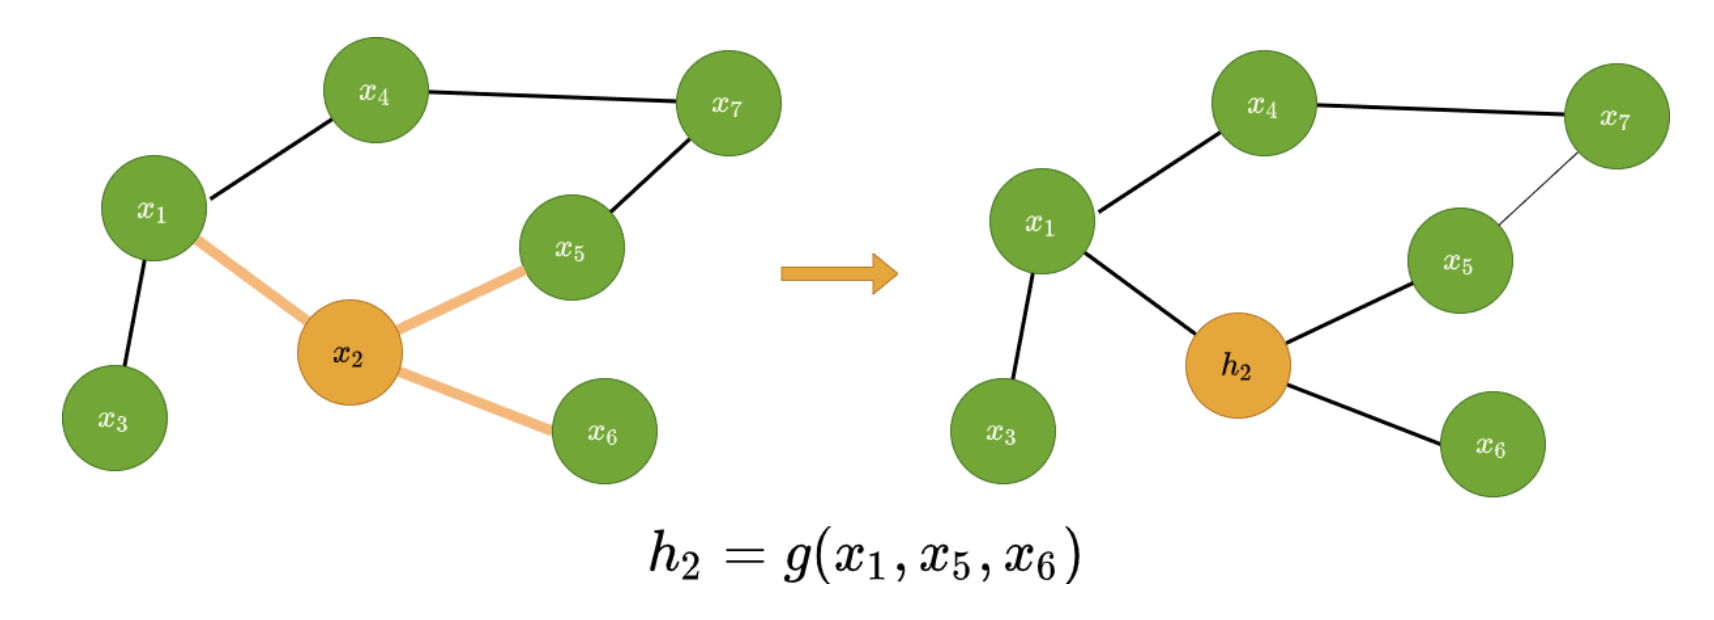
\includegraphics[width=1\textwidth]{imgs/howGNN.png}
%   \caption{A brief illustration of how Graph Neural Networks (GNN) work is presented below. The diagram is borrowed from \url{https://theaisummer.com/gnn-architectures/}}
%   \label{fig:gnn}
% \end{figure}

% Then general idea to learn the representation of congressional knowledge before joining a committee is to prepare additional nodes that encode the information of each congress, and learn the joint representation that aggregates a senator's information and those of congresses before joining such committees, as illustrated in Figure \ref{fig:daggnn}.

% \begin{figure}[h]
%   \centering
%   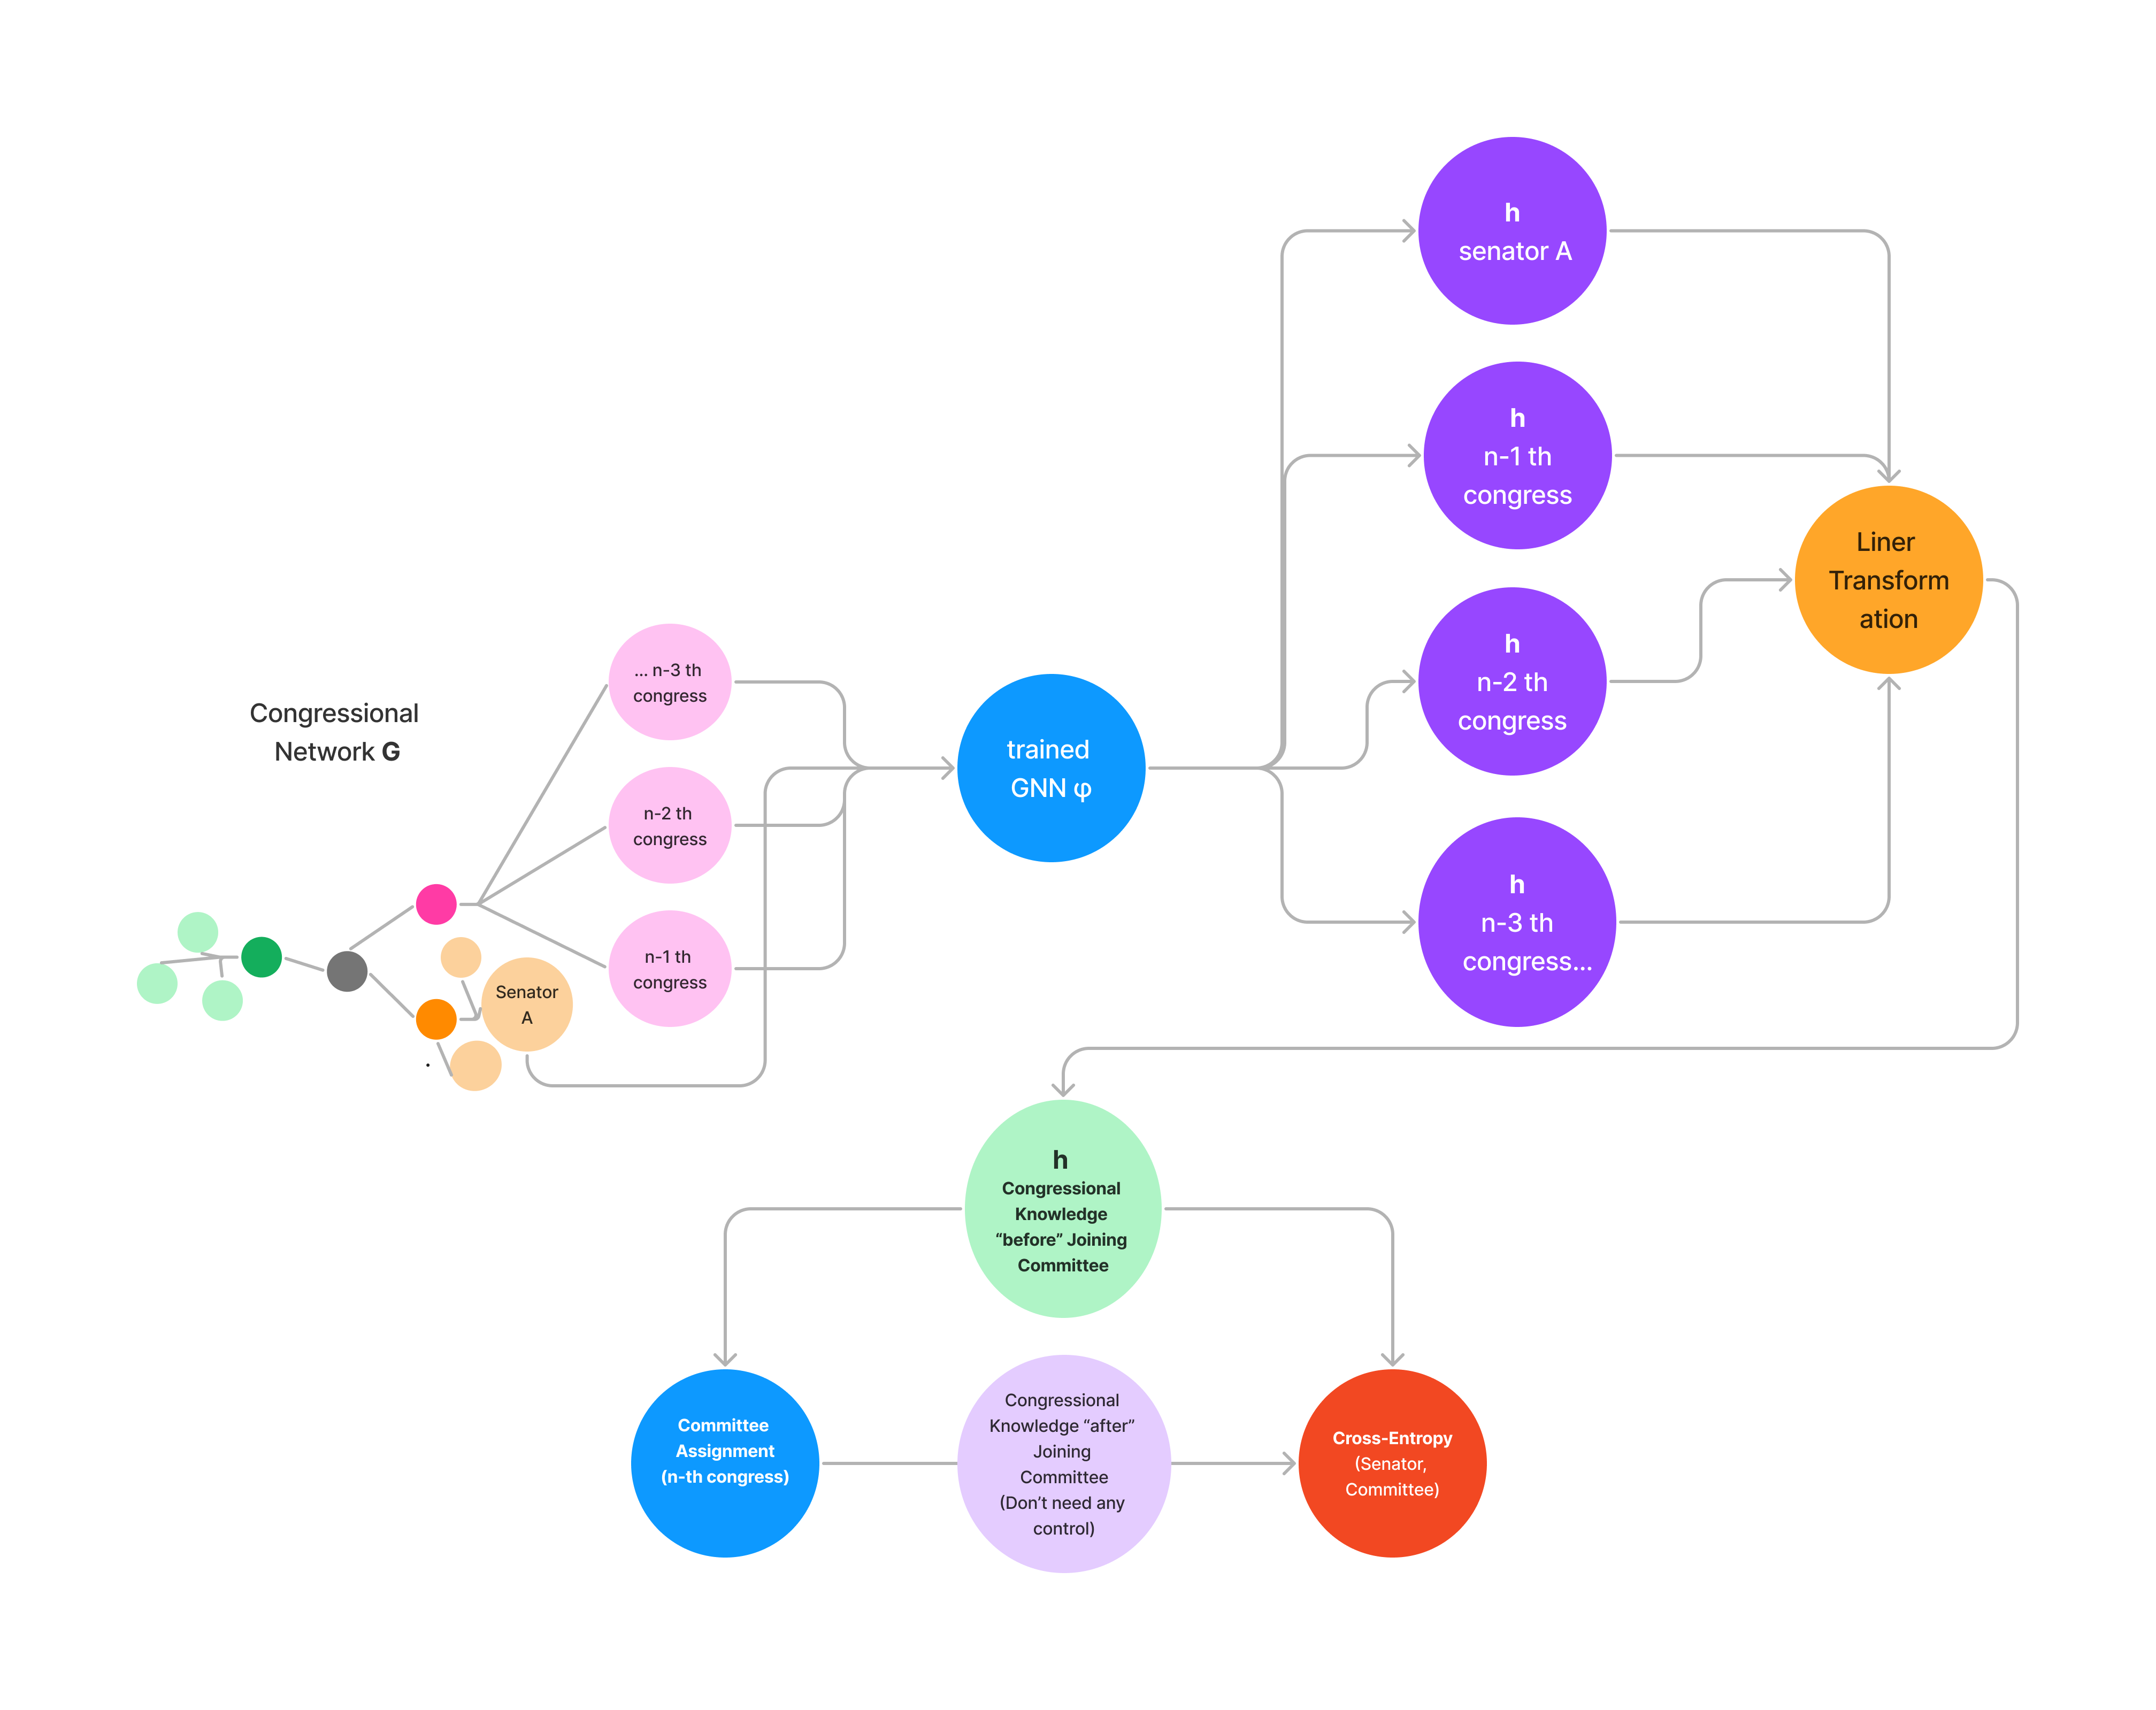
\includegraphics[width=1\textwidth]{imgs/daggnn.png}
%   \caption{An illustration of how to utilize GNN to learn the numeric representation of congressional knowledge before joining a committee}
%   \label{fig:daggnn}
% \end{figure}

% \subsection{Estimation of CATE}

% Finally, by denoting the learned representation of Senator $i$'s congressional knowledge before joining the committee at time $t$ as $h_i = \phi_{GNN}(i, G; t-1)$, the study can estimate the conditional average treatment effect (CATE) by learning estimators for both $\mu_0(h_i) \equiv \mathbb{E}\left[Y_i \mid H=h_i, T_i=0\right]$ and $\mu_1(h_i) \equiv \mathbb{E}\left[Y_i \mid H=h_i, T_i=1\right]$, and using the formula $\text{CATE}(h_i) = \mu_1(h_i) - \mu_0(h_i)$. This allows the study to estimate the effect of committee assignment on the similarity between a Senator's and the assigned committee's NAICS code distribution, while controlling for potential confounders through the learned representation $h_i = \phi_{GNN}(i, G)$.
% For the estimator $\mu_0(h_i)$ and $\mu_1(h_i)$, the study will use the Treatment Agnostic Regression Network (TARNet) \citep{tarnet}, which extends T-learners \citep{tlearner} with additional layers of neural networks that learn a shared representation of $h_i = \phi_{GNN}(i, G; t-1)$ for the treatment and control groups in a balanced way. By doing so, the neural network can effectively perform its regression task to estimate CATE, even though $h_i$ is asymmetrically distributed between the treatment and control groups.

% \begin{figure}[h]
%   \centering
%   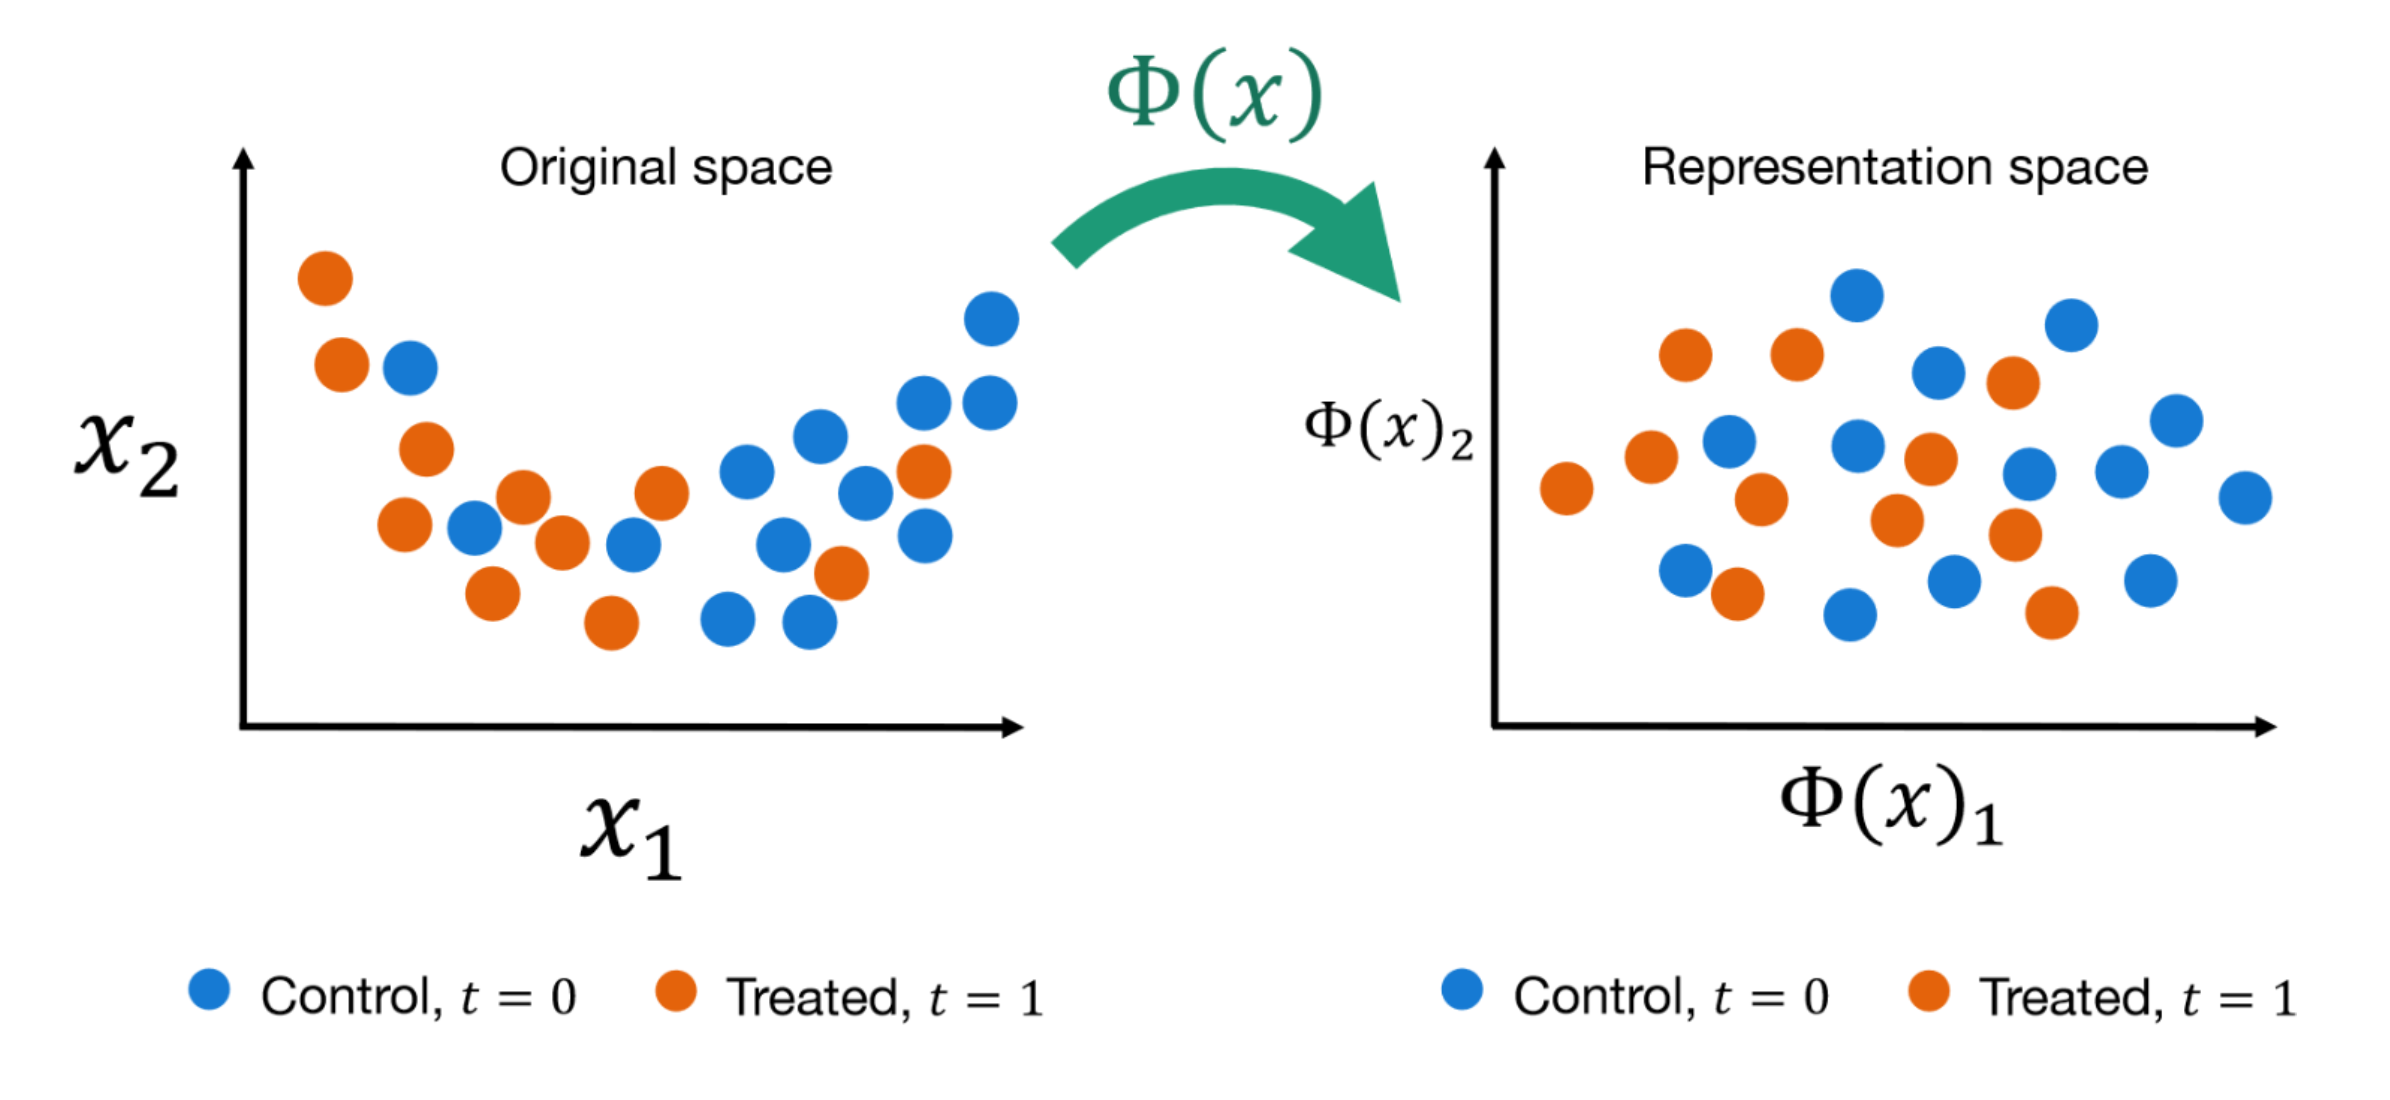
\includegraphics[width=1\textwidth]{imgs/balancing.png}
%   \caption{An illustration of how balancing works using TARNet's shared representation. The diagram is borrowed from \citep{koch}.}
%   \label{fig:bal}
% \end{figure}

% The necessity of adding an additional balancing layer is quite straightforward. For a given committee, the number of senators assigned to that committee is relatively small compared to those who are not assigned to it. By incorporating additional layers with appropriate loss functions, it is expected that $h_i$ will be mapped into a more balanced space, where $\phi_{\text{balancing}}(h_i; T=0)$ and $\phi_{\text{balancing}}(h_i; T=1)$ are evenly distributed as illustrated in Figure \ref{fig:bal}. 

% \subsection{Evaluation of CATE}
% There are a total of 62 different committees, and CATE is estimated for each committee separately using the transaction information of 95 Senators across various congresses, spanning from the 114th to the 117th Congress. By evaluating these CATE values, the paper aims to quantitatively assess how committee assignments heterogeneously affect Senators' behavior across committees and among the Senators themselves.
% \section{Conclusion and Contributions}

% The paper aims to make two main contributions. Firstly, it substantively proves the existence of insider trading by explicitly showing that committee membership changes affect Congressmen's investment behavior to become similar to the information available from the committee. Secondly, it demonstrates a novel methodological approach to estimate causal quantities using graph-structured data by leveraging representation learning via Graph Neural Network. Therefore, the paper proposes a model and learning scheme that combines a Graph Neural Network and meta-learners to learn CATE, conditioning on the output of the Graph Neural Network. 


% % From the previous section on data, I described a large network that captures congressional activities in general. Let me denote this network as $G$, which includes different types of nodes and edges as explained in Tables \ref{tab:nodes} and \ref{tab:edges}\footnote{Formally, this type of network that includes different types of nodes and edges is called a heterograph}. 

% % After analyzing the initial results, I have decided to investigate how committee membership impacts the trading behavior of Congressmen. Typically, each Congressmen is assigned to one or two committees, which are responsible for overseeing the legislation on a specific topic or bill. Companies that have a stake in the legislation have varying levels of interest and involvement, and this relationship is illustrated in Figure 2.

% % If the Lobbyview data is merged with my transaction data, it would be able to capture the 
% %  between bills, committees, companies, and Congressmen. Since these interactions can be represented as structured graph data, I plan to use a Graph Neural Network (GNN) for predictive analysis. The GNN will predict a Congressmen's investment in a specific stock using a graph network that includes information on bills, companies lobbying on those bills, committees with jurisdiction over those bills, and the Congressmen assigned to those committees.

% % A Graph Neural Network (GNN) is a type of neural network that can analyze graph-structured data. The main reason for using GNN in our research is because the data we are analyzing has a graph structure, representing different types of entities interacting with each other. Unlike traditional tabular data, graph data has a unique structure that requires a special type of model to process it. GNN can leverage the benefits of neural networks to encode complex patterns and dependencies in the graph data to effectively predict the quantity of interest, in our case the probability of stock trading of Congressmen. GNNs are also suitable for large-scale data analysis as the network involve a massive amount of data, with over 200,000 bills and 70,000 companies represented as nodes and their interactions as edges. GNNs can efficiently process such large-scale data by analyzing localized neighborhoods around each node.

% % Task-wise, I plan to use a Graph Neural Network (GNN) to perform a link prediction task. The input data will be a graph consisting of bills, companies, committees, and congressmen. The aim of the link prediction task is to predict which stock transactions are most likely to occur for a given congressman based on the interactions between these entities represented as a graph.

% % In addition, to make the GNN more interpretable, I will use a GNNExplainer \citep{gnne}, which will identify a subgraph that maximizes the mutual information with the GNN's prediction. 
% % Using the GNNExplainer will make the prediction task more interpretable, allowing us to understand how specific interactions between certain entities in the graph are likely to affect the prediction of stock transactions.
% % For example, for the prediction of Ron Wyden's semiconductor stock trading introduced in Section \ref{prelim}, I would expect GNNExplainer to provide a list of companies lobbied for CHIPS for America Act, like Samsung Electronics, Apple, Applied Materials, TSMC, QUALCOMM, Microsoft, Intel along with his committee memebership to the Senate Finance Committee as the ground of this prediction.
% % This information would help us understand why Ron Wyden made such trade.

% % \section{Conclusion}
% % The current literature lacks research on the specific information sources that lead to congressmen's stock transactions. Therefore, my research goal is to address this gap by identifying the source of information that instigated these transactions. To achieve this, I plan to merge the stock transaction data I collected with lobbyview data, which will allow me to capture the level of importance of committees to companies with lobbying activities.

% % Currently, I am merging this data and planning to use GNN for predictive analysis. However, before proceeding with deep learning using GNN, I am interested in knowing if there are other commonly used methods by political scientists to predict something with graph-structured data input. For my research, I will be using network data as input to predict each congressperson's stock trading activity.

% % Furthermore, I am seeking feedback on whether there are any ``causal-like'' estimands that can help achieve my research goal of identifying the primary source of information that congresspeople use. Currently, my approach using GNN with GNNEXplainer is purely predictive analysis and lacks a causal approach in a statistical sense. If there are any causal estimands that can help me achieve my goal, I would like to explore those avenues.

% % I have shared this research proposal with Insong, who agrees with my motivation and method. He is familiar with GNN as he has been working on a project using GNN with KAIST for over a year. I would like to know if this research direction would be persuasive for a political science paper in general.

% % Additionally, I am open to any straightforward advice to improve my research proposal. I am still in the early stages of my research, and I would appreciate any feedback to help me refine my approach. Please do not hesitate to share your thoughts.

\clearpage

\bibliography{biblo.bib}
\end{document}